\documentclass[a4paper,UKenglish,cleveref,autoref,thm-restate,numberwithinsect,final]{lipics-v2021}

\pdfoutput=1

\hideLIPIcs
\nolinenumbers

\bibliographystyle{plainurl}

\title{Learning Automata with Name Allocation}



\author{Florian Frank}%
{Friedrich-Alexander-Universität Erlangen-Nürnberg, Germany}%
{florian.ff.frank@fau.de}{https://orcid.org/0000-0002-9458-3408}%
{Supported by the Deutsche Forschungsgemeinschaft (DFG) as part of the Research and Training Group 2475 ``Cybercrime and Forensic Computing'' (393541319/GRK2475/2-2024)}

\author{Stefan Milius}
{Friedrich-Alexander-Universität Erlangen-Nürnberg, Germany}
{stefan.milius@fau.de}{https://orcid.org/0000-0002-2021-1644}
{Supported by the DFG (German Research Foundation) -- project number 419850228}

\author{Jurriaan Rot}
{Institute for Computing and Information Sciences, Radboud University, Nijmegen, the Netherlands}
{jrot@cs.ru.nl}{https://orcid.org/0000-0002-1404-6232}
{}

\author{Henning Urbat}
{Friedrich-Alexander-Universität Erlangen-Nürnberg, Germany}
{henning.urbat@fau.de}{https://orcid.org/0000-0002-3265-7168}
{Supported by the DFG (German Research Foundation) -- project number 470467389}

\authorrunning{F.~Frank, S.~Milius, J.~Rot and H.~Urbat}

\Copyright{Florian Frank, Stefan Milius, Jurriaan Rot and Henning Urbat}

\ccsdesc[500]{Theory of Computation~Formal Languages} 
\keywords{Data Languages, Nominal Sets, Languages with Binders, Automata Learning}



\usepackage[babel]{csquotes}
\usepackage{amssymb,amsmath,amsxtra,mathrsfs,mathtools,bm,stmaryrd}
\usepackage{booktabs}
\usepackage{multirow}
\usepackage{nicefrac}
\usepackage{colonequals}
\usepackage{xspace}
\usepackage{dsfont}
\usepackage{tikz}
\usetikzlibrary{arrows,arrows.meta,automata,backgrounds,calc,decorations.markings,decorations.pathreplacing,decorations.pathmorphing,fit,math,positioning,shapes,shapes.geometric,shapes.callouts,shapes.misc}
\usepackage{ifthen}
\usepackage[notref,notcite]{showkeys}
\usepackage{seqsplit}
\usepackage{xstring}
\usepackage[noadjust]{cite}
\usepackage{rotating}
\usepackage{tikz-cd}
\usepackage{blkarray}
\usepackage{adjustbox}
\usepackage{calc}
\usepackage{dutchcal}
\usepackage{etoolbox}
\usepackage{relsize}
\usepackage{microtype}
\usepackage[footnote,marginclue,nomargin,final]{fixme}

\tikzcdset{scale cd/.style={every label/.append style={scale=#1},
    cells={nodes={scale=#1}}}}

\allowdisplaybreaks


\declaretheorem[name=Definition,style=definition,numberwithin=section,sibling=definition]{defn}
\declaretheorem[name=Example,style=definition,sibling=defn]{expl}
\declaretheorem[name=Examples,style=definition,sibling=defn]{examples}
\declaretheorem[name=Observation,style=definition,sibling=defn]{obs}
\declaretheorem[name=Remark,style=definition,sibling=defn]{rem}
\declaretheorem[name=Assumptions,style=definition,sibling=defn]{assumptions}
\declaretheorem[name=Assumption,style=definition,sibling=defn]{assumption}
\declaretheorem[name=Algorithm,style=definition,sibling=defn]{algo}
\declaretheorem[name=Notation,style=definition,sibling=defn]{notation}
\declaretheorem[name=Convention,style=definition,sibling=defn]{convention}
\declaretheorem[name=Construction,style=definition,sibling=defn]{construction}
\declaretheorem[name=Theorem,style=definition,sibling=defn]{theo}
\declaretheorem[name=Research Question,style=definition,sibling=defn,numbered=no]{question}
\declaretheorem[sibling=defn]{cor}
\declaretheorem[name=Fact,style=definition,sibling=defn]{fact}
\declaretheorem[name=Lemma,style=definition,sibling=defn]{lem}
\declaretheorem[name=Proposition,style=definition,sibling=defn]{prop}
\declaretheorem[name=Proof Sketch,style=definition,sibling=defn]{proofsketch}
\declaretheorem[numbered=no,name=Theorem]{nsd}
\declaretheorem[numbered=no,name=Theorem]{reit}

\newcommand{\resetCurThmBraces}{%
\gdef\curThmBraceOpen{(}%
\gdef\curThmBraceClose{)}}
\resetCurThmBraces
\newcommand{\removeThmBraces}{%
\gdef\curThmBraceOpen{}%
\gdef\curThmBraceClose{}}
\resetCurThmBraces

\newenvironment{notheorembrackets}{\removeThmBraces}{\resetCurThmBraces}
\patchcmd{\thmhead}{(#3)}{\curThmBraceOpen #3\curThmBraceClose }{}{}

\setcounter{tocdepth}{2}

\newcommand{\defaultshowkeysformat}[1]{%
\StrSubstitute{#1}{ }{\textvisiblespace}[\TEMP]%
\parbox[t]{\marginparwidth}{\raggedright\normalfont\small\ttfamily\(\{\){\color{red!50!black}\expandafter\seqsplit\expandafter{\TEMP}}\(\}\)}%
}
\newenvironment{hideshowkeys}{%
    \renewcommand*\showkeyslabelformat[1]{%
        \noexpandarg%
    }
}{%
    \renewcommand*\showkeyslabelformat[1]{%
        \noexpandarg%
        \defaultshowkeysformat{##1}%
    }
}

\renewcommand*\showkeyslabelformat[1]{%
\noexpandarg%
\defaultshowkeysformat{#1}%
}

\renewcommand\itemautorefname{Item}
\newcommand{\itemref}[2]{\autoref{#1}.\ref{#2}}

\newcommand{\mypar}[1]{%
    \subparagraph*{#1.}%
}


\newcommand\restr[2]{{%
  \left.\kern-\nulldelimiterspace %
  #1 %
  \littletaller %
  \right|{}^{#2} %
}}

\DeclareMathOperator{\norb}{\sharp_o}
\DeclareMathOperator{\Sub}{\mathsf{Sub}}
\DeclareMathOperator{\dom}{\textsf{dom}}
\DeclareMathOperator{\supp}{\mathsf{supp}}
\DeclareMathOperator{\repr}{\textsf{repr}}
\DeclareMathOperator{\im}{\textsf{im}}
\DeclareMathOperator{\coim}{\textsf{coim}}
\DeclareMathOperator{\alphaequiv}{\equiv_{\alpha}}
\DeclareMathOperator{\alphanequiv}{{\not\equiv}_{\alpha}}
\DeclareMathOperator{\fix}{\textsf{fix}}
\DeclareMathOperator{\Fix}{\textsf{Fix}}
\DeclareMathOperator{\isf}{\trianglelefteqslant}

\newcommand{\littletaller}{\mathchoice{\vphantom{\big|}}{}{}{}}

\newcommand{\seq}{\subseteq}
\newcommand{\qes}{\supseteq}
\newcommand{\fseq}{\seq_{\textsf{f}}}
\newcommand{\xra}[1]{\xrightarrow{#1}}
\newcommand{\xla}[1]{\xleftarrow{#1}}
\newcommand{\xto}[1]{\xra{#1}}

\newcommand{\mar}{\ar[rightarrowtail]}
\newcommand{\ear}{\ar[two heads]}

\newcommand{\deriv}[2]{{#1}^{-1}#2}
\newcommand{\Der}{\mathsf{Der}}

\newcommand{\muBar}{\textsf{Bar-$\mu$TL}\xspace}

\newcommand{\smooth}{smooth\xspace}
\newcommand{\opcit}[1][.]{\textit{op.cit#1}\xspace}

\newcommand{\At}{\mathds{A}}
\newcommand{\Sigmas}{\Sigma^{\star}}
\newcommand{\Ats}{\At^{\!\raisebox{1pt}{\scriptsize$\star$}}}
\newcommand{\Atw}{\At^{\omega}}
\newcommand{\barAs}{\barNames^{\star}}
\newcommand{\barAw}{\barNames^{\omega}}
\newcommand{\barAwfs}{\barNames^{\omega}_{\textsf{fs}}}
\newcommand{\ol}{\overline}
\def\ul{\underline}

\newcommand{\bars}{\mathsf{bs}}

\newcommand{\sem}[1]{\llbracket #1 \rrbracket}

\newcommand{\op}[1]{\operatorname{\mathsf{#1}}}
\newcommand{\id}{\op{id}}

\newcommand{\inj}{\op{in}}
\newcommand{\inl}{\op{inl}}
\newcommand{\inr}{\op{inr}}
\newcommand{\pr}{\op{pr}}
\newcommand{\kan}{\op{kan}}
\newcommand{\cl}{\op{cl}}
\newcommand{\nd}{\op{nd}}
\newcommand{\rest}{\op{rest}}
\newcommand{\gdw}{\Leftrightarrow}
\newcommand{\lgdw}{\Longleftrightarrow}

\newcommand{\Jir}{\mathsf{JI}}

\newcommand{\card}[1]{\left\vert#1\right\vert}
\let\abs\card

\newcommand{\formu}{\textsf{form}}

\newcommand{\SUC}{\mathfrak{N}}

\newcommand{\states}{\mathsf{s}}
\newcommand{\al}{\mathsf{a}}
\newcommand{\trans}{\mathsf{t}}
\newcommand{\init}{\mathsf{i}}
\newcommand{\final}{\mathsf{f}}

\newcommand{\A}{\mathcal{A}}
\renewcommand{\H}{\mathcal{H}}

\newcommand{\can}[2]{\mathsf{can}_{#1}^{#2}}

\newcommand{\canmap}{\mathsf{can}}

\newcommand{\allbool}{\mathcal{B}}
\newcommand{\posbool}{\allbool_+}
\newcommand{\pos}[1]{{#1}^{+}}
\newcommand{\negsym}{\mathsf{n}}
\newcommand{\negstate}[1]{#1_{\negsym}}
\newcommand{\negbool}{\allbool_{\negsym}}
\newcommand{\dualbool}{\allbool_\mathsf{d}}
\newcommand{\dual}[1]{{#1}^\mathsf{d}}
\newcommand{\graph}{\mathcal{G}}
\newcommand{\tree}{\mathcal{T}}
\newcommand{\reachtree}[3]{\mathcal{R}_{#1}^{#2}(#3)}

\newcommand{\teach}{\textsf{T}\xspace}
\newcommand{\learn}{\textsf{L}\xspace}
\newcommand{\tass}{\textsf{TA}\xspace}
\newcommand{\corproc}{\textsf{CoR}\xspace}

\newcommand{\bartree}[1][\barNamess]{\mathcal{T}_{#1}}
\newcommand{\datatree}[1][\names]{\mathcal{T}_{#1}}

\newcommand{\rsem}{\vDash^{\textsf{r}}}

\newcommand{\cat}[1]{\mathscr{#1}}
\def\A{\cat A}
\def\B{\cat B}
\def\C{\cat C}
\def\D{\cat D}
\newcommand{\E}{\mathcal{E}}
\newcommand{\II}{\mathbb{I}}
\newcommand{\FF}{\mathbb{F}}
\newcommand{\MM}{\mathcal{M}}
\newcommand{\Set}{\mathbf{Set}}
\newcommand{\Pos}{\mathsf{Pos}}
\newcommand{\Pfn}{\mathsf{Pfn}}
\newcommand{\Gra}{\mathsf{Gra}}
\newcommand{\KVec}{K\text{-}\mathsf{Vec}}
\newcommand{\CPO}{\mathsf{CPO}}
\newcommand{\DCPO}{\mathsf{DCPO}}
\newcommand{\DCPOb}{\mathsf{DCPO}_\bot}
\newcommand{\CMS}{\mathsf{CMS}}
\newcommand{\MS}{\mathsf{MS}}
\newcommand{\Ord}{\mathsf{Ord}}
\newcommand{\Presheaf}[1]{\Set^{#1}}

\newcommand{\Pow}{\mathcal{P}}
\newcommand{\Powf}{\Pow_\mathsf{f}} %

\newcommand{\M}{\mathcal{M}}

\newcommand{\NAut}{\mathbf{NAut}}
\newcommand{\NAutfp}{\mathbf{NAut}_{\mathsf{fp}}}

\newcommand{\N}{\mathds{N}}
\newcommand{\R}{\mathds{R}}
\newcommand{\Z}{\mathds{Z}}
\newcommand{\fpair}[1]{\ensuremath{\langle #1 \rangle}}

\renewcommand{\epsilon}{\varepsilon}

\newcommand{\Coalg}{\mathop{\mathsf{Coalg}}}
\newcommand{\Alg}{\mathop{\mathsf{Alg}}}
\newcommand{\colim}{\mathop{\mathsf{colim}}}

\def\variety{variety\xspace}
\def\varieties{varieties\xspace}
\def\eqnth{equational theory\xspace}
\def\eqnths{equational theories\xspace}
\def\Eq{\mathbb{E}}

\renewcommand{\S}{\mathscr{S}}
\renewcommand{\P}{\mathbb{P}}
\newcommand{\K}{\mathds{K}}

\newcommand{\reg}{{\mathrm{reg}}}

\newcommand\epidownarrow{\mathrel{\rotatebox[origin=c]{90}{$\twoheadleftarrow$}}}

\newcommand{\Nom}{\mathbf{Nom}}
\newcommand{\RnNom}{\mathbf{RnNom}}
\newcommand{\orb}{\mathsf{orb}}
\newcommand{\Perm}{\mathsf{Perm}}
\newcommand{\names}{\At}
\newcommand{\Abstr}[2][\names]{[#1]#2}
\newcommand{\datalang}{\powfs(\names^*)}
\newcommand{\parnom}[1]{\names^{\$\mathbf{#1}}}
\newcommand{\compr}{:}
\newcommand{\ufs}{{\mathsf{ufs}}}
\newcommand{\braket}[1]{\langle #1 \rangle}
\newcommand{\fs}{\mathsf{fs}}
\newcommand{\pow}{\mathcal{P}}
\newcommand{\powf}{\pow_{\omega}}
\newcommand{\powufs}{\pow_{\ufs}}
\newcommand{\powfs}{\pow_{\fs}}
\newcommand{\pown}[1]{\pow_{\leqslant #1}}
\newcommand{\fresh}{\mathbin{\#}}

\newcommand{\MSOep}{\text{MSO}^{\sim,+}}
\newcommand{\MSOe}{\text{MSO}^{\sim}}

\renewcommand{\Eq}{\mathsf{Eq}}
\renewcommand{\phi}{\varphi}

\newcommand{\lfp}{locally finitely presentable\xspace}
\newcommand{\lcp}{locally cofinitely presentable\xspace}
\newcommand{\lfs}{locally finitely super-presentable\xspace}


\newcommand{\beh}{\mathsf{beh}}
\newcommand{\hookto}{\hookrightarrow}
\newcommand{\subto}{\hookto}
\newcommand{\epito}{\twoheadrightarrow}
\newcommand{\epiot}{\twoheadleftarrow}
\newcommand{\ot}{\leftarrow}
\newcommand{\up}{\uparrow}
\newcommand{\ddown}{\twoheaddownarrow}
\newcommand{\sdown}{\twoheaddownarrow_s}
\newcommand{\down}{\downarrow}
\newcommand{\downinj}{\downarrowtail}
\newcommand{\monoto}{\rightarrowtail}
\newcommand{\sqleq}{\sqsubseteq}
\newcommand{\cleq}{\trianglelefteq}
\newcommand{\nsqleq}{\nsqsubseteq}
\newcommand{\pto}{\rightharpoonup}
\newcommand{\MB}{\mathbf{B}}

\newcommand{\f}{\mathsf{f}}
\newcommand{\nf}{\ensuremath{\mathsf{nf}}}

\newcommand{\fin}{\nu}
\newcommand{\ter}{\tau}
\newcommand{\ini}{\iota}
\newcommand{\inic}{\mu}

\newcommand*\cocolon{%
        \nobreak
        \mskip6mu plus1mu
        \mathpunct{}%
        \nonscript
        \mkern-\thinmuskip
        {:}%
        \relax
}

\newcommand{\set}[1]{\{#1\}}
\newcommand{\setw}[2]{\{#1\,\mid\,#2\}}

\newcommand{\Abar}{B}
\newcommand{\dbar}{d'}
\newcommand{\eps}{\varepsilon}
\newcommand{\opp}{\mathsf{op}}

\newcommand{\Lstar}{$\mathsf{L}^{\ast}$\xspace}
\newcommand{\Lsharp}{$\mathsf{L}^{\#}$\xspace}
\newcommand{\NLstar}{$\mathsf{NL}^{\ast}$\xspace}
\newcommand{\nomLstar}{$\nu\mathsf{L}^{\ast}$\xspace}
\newcommand{\nomNLstar}{$\nu\mathsf{NL}^{\ast}$\xspace}

\newcommand{\mhat}{\widehat{m}}
\newcommand{\ehat}{\widehat{e}}
\newcommand{\chat}{\widehat{c}}  
\renewcommand{\o}{\cdot}

\newcommand{\takeout}[1]{\empty}


\newcommand{\descto}[3][]{\arrow[phantom]{#2}[#1]{\text{\footnotesize{}\begin{tabular}{c}#3\end{tabular}}}}
\newcommand{\desctox}[4][]{\arrow[phantom,#2]{#3}[#1]{\text{\footnotesize{}\begin{tabular}{c}#4\end{tabular}}}}

\tikzset{shiftarr/.style={
        rounded corners,%
        to path={--([#1]\tikztostart.center)
                     -- ([#1]\tikztotarget.center) \tikztonodes
                     -- (\tikztotarget)},
}}

\tikzset{shiftarrr/.style={
        rounded corners,%
        to path={-- ([#1]\tikztostart.center)
                    |- (\tikztotarget)  \tikztonodes},
}}

\tikzset{roundcornerarr/.style={
        rounded corners,%
        to path={--([#1]\tikztostart.south)
                     |- (\tikztotarget) \tikztonodes},
}}

\tikzset{roundcornerarrr/.style={
        rounded corners,%
        to path={ -| (\tikztotarget) \tikztonodes},
}}

\tikzset{roundcornerarrrr/.style={
        rounded corners,%
        to path={ |- (\tikztotarget) \tikztonodes},
}}

\newcommand{\pullbackangle}[2][]{\arrow[phantom,to path={
                     -- ($ (\tikztostart)!1cm!#2:([xshift=8cm]\tikztostart) $)
                        node[anchor=west,pos=0.0,rotate=#2,
                        inner xsep = 0]
                        {\begin{tikzpicture}[minimum
                        height=1mm,baseline=0,#1]
    \draw[-] (0,0) -- (.5em,.5em) -- (0,1em);
                        \end{tikzpicture}}}]{}}

\newcommand{\overbar}[1]{\mkern 1.5mu\overline{\mkern-1.5mu#1\mkern-1.5mu}\mkern 1.5mu}

\newcommand{\mybar}[3]{%
  \mathrlap{\hspace{#2}\overline{\scalebox{#1}[1]{\phantom{\ensuremath{#3}}}}}\ensuremath{#3}
}

\newcommand{\myhat}[3]{%
  \mathrlap{\hspace{#2}\widehat{\scalebox{#1}[1]{\phantom{\ensuremath{#3}}}}}\ensuremath{#3}
}

\newcommand{\FN}{\mathsf{FN}}
\newcommand{\BN}{\mathsf{BN}}
\newcommand{\RN}{\mathsf{RN}}
\newcommand{\NA}{\mathsf{N}}
\newcommand{\VAR}{\mathsf{V}}
\newcommand{\FV}{\mathsf{FV}}
\newcommand{\fp}{\mathsf{fp}}
\newcommand{\Lpre}{L_{\mathsf{pre}}}

\newcommand{\BarForm}{\mathsf{Bar}}

\newcommand{\barA}{{\mybar{0.6}{2.5pt}{A}}} %
\newcommand{\barF}{\mybar{0.6}{2.5pt}{F}}
\newcommand{\barG}{\mybar{0.6}{2pt}{G}}
\newcommand{\barI}{\mybar{0.6}{2pt}{I}}
\newcommand{\barJ}{\mybar{0.6}{2pt}{J}}
\newcommand{\barE}{\mybar{0.6}{2.5pt}{E}}

\newcommand{\bark}{\mybar{0.7}{1.5pt}{k}}

\newcommand{\barL}{\mybar{0.8}{1.5pt}{L}}
\newcommand{\barR}{\mybar{0.8}{2pt}{R}}

\newcommand{\barQ}{\mybar{0.7}{2pt}{Q}}
\newcommand{\barDelta}{\mybar{0.6}{2pt}{\delta}}
\newcommand{\barNames}{{\mybar{0.55}{1.6pt}{\names}}}
\newcommand{\barAscript}{{\overbar{A}}}
\newcommand{\barNamess}{{\overbar{\names}}}


\newcommand{\barGF}{\mybar{0.85}{2pt}{GF}}
\newcommand{\barFpG}{\mybar{0.9}{2pt}{F + G}}
\newcommand{\barFtG}{\mybar{0.9}{2pt}{F \times G}}
\newcommand{\barAbs}{\mybar{0.8}{1.5pt}{[\names]}}

\newcommand{\hatF}{\widehat{F}}
\newcommand{\hatG}{\widehat{G}}
\newcommand{\hatGF}{\myhat{0.9}{2pt}{GF}}

\newcommand{\ngt}{{\mathsf{ngt}}}
\newcommand{\rg}{{\mathsf{rg}}}
\renewcommand{\ng}{{\mathsf{ng}}}
\newcommand{\fsuba}{{\mathsf{fsuba}}}
\newcommand{\ub}{{\mathsf{ub}}}

\newcommand{\lan}{\ddagger}
\newcommand{\dsS}{\mathds{S}}

\newcommand{\Lan}{\textsf{Lan}}
\newcommand{\Run}{\textsf{AccRun}}
\newcommand{\oRun}{\overline{\textsf{Run}}}
\newcommand{\Ran}{\textsf{Ran}}

\newcommand{\runtree}{\textsf{run}}


\newcommand{\Var}{\mathsf{Var}}
\newcommand{\Fin}{\mathsf{Fin}}
\newcommand{\Field}{\mathds{Z}}
\newcommand{\AlgSigma}{\mathbb{\Sigma}}
\newcommand{\AlgEqns}{\mathbb{E}}
\newcommand{\Nat}{\mathds{N}}
\newcommand{\Int}{\mathds{Z}}
\newcommand{\Real}{\mathds{R}}
\newcommand{\Rat}{\mathds{Q}}
\newcommand{\balpha}{{\boldsymbol \alpha}}
\newcommand{\bgamma}{{\boldsymbol \gamma}}

\newcommand{\Eloise}{\ensuremath{\exists}\text{loise}\xspace}
\newcommand{\Abelard}{\ensuremath{\forall}\text{bélard}\xspace}
\newcommand{\EloiseShort}{\ensuremath{\exists}}
\newcommand{\AbelardShort}{\ensuremath{\forall}}
\newcommand{\SubForm}{\mathbb{S}}
\newcommand{\Player}{\ensuremath{\mathfrak{p}}}
\newcommand{\CPlayer}[1][\Player]{\ensuremath{\overline{#1}}}
\newcommand{\Players}{\ensuremath{\mathbb{P}}}

\newcommand{\AccGame}[1][]{\ensuremath{\Game^{\textsf{Acc}}_{\mkern-3mu #1}}}
\newcommand{\RANAFunc}{\ensuremath{\mathbcal{A}}}
\newcommand{\ComArr}{\mathlarger{\mathlarger{\mathlarger{\mathbf{\circlearrowleft}}}}}

\newcommand{\one}{\mathbf{1}}
\newcommand{\bone}{{\bf 1}}
\newcommand{\bb}{{\bf b}}
\newcommand{\bu}{{\bf u}}
\newcommand{\bv}{{\bf v}}
\newcommand{\bs}{{\bf s}}

\newcommand{\wordlang}[1]{\ensuremath{\mathsf{W}(#1)}}
\newcommand{\prelang}[1]{\ensuremath{\mathsf{P}(#1)}}


\newcommand{\longmid}{\hspace{0.9ex}\smash{\rule[-1.0ex]{0.41pt}{3.2ex}}\hspace{0.9ex}}
\newcommand{\midmid}{\hspace{0.2ex}{\rule[-0.1ex]{0.6pt}{1.65ex}}\hspace{0.2ex}}
\newcommand{\scriptmidmid}{\hspace{0.2ex}{\rule[-0.1ex]{0.6pt}{1.1ex}}\hspace{0.2ex}}
\newcommand{\subscriptmidmid}{\hspace{0.2ex}{\rule[-0.1ex]{0.6pt}{0.9ex}}\hspace{0.2ex}}

\newcommand{\newletter}[1]{{\midmid}#1}
\newcommand{\scriptnew}[1]{{\scriptmidmid}#1}
\newcommand{\subscriptnew}[1]{{\subscriptmidmid}#1}
\newcommand{\newtreeletter}[1]{{\nu}#1}

\newcommand{\quotient}[2]{{#1}/{#2}} %

\let\originalleft\left
\let\originalright\right
\renewcommand{\left}{\mathopen{}\mathclose\bgroup\originalleft}
\renewcommand{\right}{\aftergroup\egroup\originalright}

\ExplSyntaxOn
\NewDocumentCommand{\makecycle}{om}{
	\ensuremath{ \left(~\guest_print_list:nn { #2 } {~{\ }~}~\right)\IfValueT{#1}{^{#1}}}
}
\NewDocumentCommand{\maketuple}{om}{%
\ensuremath{\left(~\guest_print_list:nn { #2 } {~{,\:}~}~\right)\IfValueT{#1}{^{#1}}}
}
\NewDocumentCommand{\makemonad}{om}{
	\ensuremath{ \left\langle~\guest_print_list:nn { #2 } {~{,\ }~}~\right\rangle\IfValueT{#1}{^{#1}}}
}
\NewDocumentCommand{\makegrammar}{om}{
	\ensuremath{ ~\guest_print_list:nn { #2 } {~{\ \,\vert\ \,}~}~\IfValueT{#1}{^{#1}}}
}

\seq_new:N \l_guest_list_seq
\cs_new_protected:Nn \guest_print_list:nn
{
	\seq_set_from_clist:Nn \l_guest_list_seq { #1 }
	\seq_use:Nn \l_guest_list_seq { #2 }
}
\ExplSyntaxOff

\usepackage[noend]{algpseudocode}
\renewcommand{\algorithmicrequire}{\textbf{Input:}}
\algrenewcommand{\algorithmiccomment}[1]{\hfill// #1}

\usepackage{hyperref}
\hypersetup{hidelinks,final,bookmarks}

\addto\extrasUKenglish{%
    \renewcommand{\subsectionautorefname}{Section}
}


\FXRegisterAuthor{ff}{aff}{FF} %
\FXRegisterAuthor{sm}{asm}{SM} %
\FXRegisterAuthor{hu}{ahu}{HU} %
\FXRegisterAuthor{jr}{ajr}{JR} %

\begin{document}
    \maketitle
    \begin{abstract}
      Automata over infinite alphabets have emerged as a convenient computational model for processing structures involving data, such as nonces in cryptographic protocols or data values in XML documents. We introduce active learning methods for \emph{bar automata}, a species of automata that process finite data words represented as bar strings, which are words with explicit name binding letters. Bar automata have pleasant algorithmic properties. We develop a framework in which \emph{every} learning algorithm for standard deterministic or nondeterministic finite automata over finite alphabets can be used to learn bar automata, with a query complexity determined by that of the chosen learner. The technical key to our approach is the algorithmic handling of $\alpha$-equivalence of bar strings, which allows to bridge the gap between finite and infinite alphabets. The principles underlying our framework are generic and also apply to bar Büchi automata and bar tree automata, leading to the first active learning methods for data languages of infinite words and finite trees.
      \end{abstract}
      
    \section{Introduction}\label{sec:intro}
	
	Active automata learning is a family of techniques for inferring an automaton from a black-box system, by interacting with this system and making observations about its behaviour. 
	Originally introduced by Angluin~\cite{angluin87}, the celebrated \Lstar algorithm allows to effectively learn deterministic finite automata in this way. Since her work, automata learning has been combined with model checking and conformance testing techniques~\cite{DBLP:journals/jalc/PeledVY02}, turning it into an effective tool for bug finding. Indeed, automata learning algorithms have been used to analyze and learn models of network protocols (e.g.~\cite{DBLP:conf/ndss/Fiterau-Brostean23,FiterauEtAl17,FJV16}), legacy code~\cite{AslamCSB20,SHV16}, embedded software~\cite{SmeenkMVJ15} and interfaces of software components~\cite{HowarISBJ12}; see~\cite{DBLP:journals/cacm/Vaandrager17,HowarS16} for further references.
	
In addition, Angluin's original \Lstar algorithm has been improved in various ways. State-of-the-art algorithms such as $\mathsf{TTT}$~\cite{ihs14} and \Lsharp~\cite{vgrw22} may substantially reduce the number of
queries needed during learning. Orthogonally there have been numerous extensions of \Lstar-type
algorithms to models beyond classical deterministic finite automata, including for example nondeterministic finite automata~\cite{bhkl09}, Mealy machines~\cite{MargariaNRS04}, quantitative automata~\cite{bm15,hkrs20},
tree automata~\cite{dh03,k13}, automata for languages of infinite
words~\cite{af16,MalerP95,fcctw08,lczl21}, and, most relevant for this paper, automata over infinite alphabets, namely register automata~\cite{DBLP:conf/tacas/DierlFHJST24,CasselHJS16,CEGAR12,BolligHLM13}, data automata~\cite{dhlt14} and nominal automata~\cite{mssks17,ms22}. Infinite alphabets represent data, for
example, nonces in cryptographic protocols~\cite{KurtzEA07}, data
values in XML documents~\cite{NevenEA04}, object
identities~\cite{GrigoreEA13}, or parameters of method
calls~\cite{HowarEA19}. The principal challenge for all learning algorithms for data languages is to cleverly represent infinite data by finite means.

In the present paper, we study the theoretical and algorithmic aspects of active learning of \emph{bar automata}, a species of non-deterministic automata for data languages introduced in recent years in versions for finite data words (\emph{bar word automata})~\cite{skmw17}, infinite data words (\emph{bar Büchi automata})~\cite{uhms21} and finite data trees (\emph{bar tree automata})~\cite{ps24}. Bar automata yield a finite representation of corresponding nominal models with explicit name allocation, namely regular non-deterministic nominal automata (RNNAs)~\cite{skmw17}, Büchi RNNAs~\cite{uhms21} and regular non-deterministic nominal tree automata (RNTAs)~\cite{uhms21}, respectively. For Büchi RNNAs and RNTAs, these exact correspondences are new results (\Cref{thm:bar-vs-rnna}), and the constructions underlying the proof will feature crucially in our learning algorithms.

The key difference between bar automata and other models for data languages, such as non-deterministic register automata~\cite{KaminskiFrancez94,KaminskiZeitlin10} or the equivalent non-deterministic nominal orbit-finite automata~\cite{BojanczykEA14}, is the use of \emph{binding transitions} while at the same time restricting to {finite} (rather than orbit-finite) branching. In this way, bar automata retain a reasonable level of expressivity; they correspond to a proper subclass of non-deterministic register automata and are incomparable to deterministic ones. The central feature of bar automata are their very pleasant algorithmic properties: most notably, the language inclusion problem is decidable in space
polynomial in the size of the automata and exponential in their \emph{degree}, which corresponds
to the number of registers. This is in sharp constrast to standard non-deterministic register automata where inclusion is undecidable for automata with more than two registers~\cite{KaminskiFrancez94} (or one register in terms of the definition by Demri und Lazi\'c~\cite{DemriLazic09}). 

The standard semantics of bar automata is at the level of \emph{bar languages}. For instance, bar word automata consume \emph{bar strings}, which are finite words formed from \emph{plain letters} $a$ and \emph{bar letters} $\newletter a$ with $a$ taken from an infinite domain $\names$ of names (representing data values). Intuitively, a bar string
is a pattern that determines how letters are read from the input and
stored in memory for future comparison, where an occurrence of $\newletter a$ is interpreted as
reading an input letter and binding this letter to the name $a$. Accordingly, bar word languages are
sets of bar strings modulo an obvious notion of $\alpha$-equivalence induced by capture avoiding
renaming of bound letters. Bar word languages can be interpreted as data word languages (i.e.~sets of words over $\names$ without bar letters) in two ways corresponding to two slightly different disciplines of $\alpha$-renaming of bound names: \emph{global freshness} means that binding transitions read names which have not occured before (as in session automata~\cite{BolligEA14}), and \emph{local freshness} means that names are not currently stored in memory (as in register automata).
Similar principles apply to bar languages of infinite bar strings and bar trees, which are trees over a finite signature where every symbol is annotated with a bar/plain letter.

Our main contribution is an active learning method for bar automata that applies {uniformly} to bar word, bar Büchi and bar tree automata.
More specifically, we demonstrate that \emph{any} learning algorithm for classical automata over
(in)finite words or trees can be extended to a learning algorithm for the associated type of
bar automata; our extension is agnostic to the
choice of the underlying learning algorithm. The key technical idea to our approach is to reduce the problem of
learning an unknown bar language to learning a canonical representation over a restricted, finite
subalphabet. This representation, whose language is closed under
$\alpha$-equivalence w.r.t.~to the finite subalphabet, is itself a regular language over a
finite alphabet, making it amenable to classical learning.

However, this reduction is far from immediate: there is a mismatch in the types of counterexamples that the learner receives. To see this, let us recall Angluin's \emph{minimally adequate teacher} (MAT)
framework, which allows the learner to pose membership queries (`is this input in the language?') and equivalence queries (`is this hypothesis automaton $\H$ correct?') to an oracle. For equivalence queries,
the oracle returns a counterexample whenever $\H$ is incorrect. This is precisely where the difficulty lies: this counterexample may not be useful to learn
the canonical representation of the language over the subalphabet.

The core ingredient to match these counterexamples and resolve this mismatch is to effectively
find $\alpha$-equivalent words over the subalphabet. We therefore introduce new techniques for
checking $\alpha$-equivalence of (in)finite bar strings and bar trees.
Our
methods for deciding $\alpha$-equivalence are non-trivial and, moreover, of independent
interest, as they do not just arise in automata learning but potentially also in other
algorithms handling bar automata, such as minimization, reduction, or model checking.  By combining these
techniques for $\alpha$-equivalence and our reductions with known algorithms for learning
word/tree automata or automata over infinite words, we thus obtain learning algorithms for bar
languages over each of these variants. By learning bar automata and interpreting them under local or global freshness semantics, our algorithms can be understood as learning data languages. The classes of data languages learnable in this way are incomparable to existing learning algorithms for register or nominal automata; see `Related Work' below and \Cref{sec:bar-automata}. 

In summary, the main contributions of this paper are twofold:
(1) We give a reduction of the problem of learning bar automata to that of learning classical automata for regular languages of finite words, infinite words, or finite trees; and (2) we develop an approach for effectively
checking $\alpha$-equivalence of finite and infinite bar strings as well as bar trees.



    



\mypar{Related Work} Learning automata models for data languages of finite words without explicit binding is an active area of research.
 Bollig et al.~\cite{BolligHLM13} introduced
a learning algorithm for \emph{session automata}, which are register automata requiring some
data values to be \emph{fresh} for the whole string. They are equivalent to a subclass of bar
word automata under global freshness~\cite{skmw17}.  Their learning
algorithm %
uses a somewhat similar idea to ours in that it reduces the learning problem to the \Lstar algorithm for deterministic
finite automata. Our algorithm can learn a non-deterministic, hence more succinct representation of session automata.

Cassel et al.~\cite{CasselHJS16} and Dierl et al.~\cite{DBLP:conf/tacas/DierlFHJST24} learn \enquote{determinate} register automata on finite words, which are semantically equivalent to deterministic ones and are incomparable to bar automata under local freshness.
Similarly, Aarts et al.~\cite{afkv15} learn deterministic register automata with outputs which are again incomparable to bar automata under local freshness.
Moerman et al.~\cite{mssks17,ms22} present learning algorithms for deterministic nominal automata as well as for \emph{residual} non-deterministic nominal automata on finite
words. Residual nominal automata are incomparable to bar automata under local freshness (\Cref{ex:nonresidual}).

To the best of our knowledge, there is no prior work on learning either Büchi or tree data
languages. Our contributions yield learning algorithms for subclasses of both kinds.

 \section{Active Automata Learning}\label{sec:active-learning} Automata learning is about systematically inferring an automaton for an
    \emph{unknown} language~$L_\teach$. Most approaches are based on Angluin's framework~\cite{angluin87} of a \emph{minimally adequate teacher} (MAT), a game between a \emph{learner} that aims to infer $L_\teach$, and a \emph{teacher} that the learner can ask for pieces of information about $L_\teach$. To this end, the learner runs an algorithm generating a sequence $\H_1,\H_2,\H_3,\ldots$ of automata (\emph{hypotheses}) that yield increasingly improved approximations of $L_\teach$. To improve the current hypothesis $\H_i$, the learner can direct two types of questions to the teacher: \emph{membership queries} (`is a given input in $L_\teach$?') and \emph{equivalence queries} (`is the hypothesis $\H_i$ correct, i.e.~accepting $L_\teach$?'). The teacher's reply to an equivalence query is either 'Yes', in which case the learner has successfully inferred $L_\teach$, or a \emph{counterexample}, that is, an input on which $\H_i$ and $L_\teach$ differ. Note that inputs of membership queries are chosen by the learner, making this setting \emph{active}. In contrast, in \emph{passive} learning only a fixed set of  examples of elements and non-elements of $L_\teach$ is given. Active learning has been studied for numerous automata models. We consider three cases:

\mypar{Finite Automata} A \emph{(non-)deterministic finite automaton} (\emph{DFA}/\emph{NFA}) $\A = (Q, A, \to, q_0, F)$ is given by a finite set $Q$ of states, a finite input alphabet $A$, an initial state $q_0\in Q$, final states $F\seq Q$ and a transition relation $\to\,\seq Q\times A\times Q$, which in the deterministic case forms a function from $Q\times A$ to $Q$. The \emph{language $L_0(\A)\seq A^*$ accepted by $\A$} is the set of all finite words $w=a_1\cdots a_n$ for which there exists an accepting run, that is, a sequence of transitions $q_0\xto{a_1} q_1\xto{a_2}\cdots \xto{a_n} q_n$ ending in a final state. Languages accepted by finite automata are called \emph{regular}. In MAT-based learning algorithms for finite automata, one assumes an unknown regular language $L_\teach\seq A^*$ (with known alphabet $A$) and admits the learner to put the following types of queries to the teacher:
    \begin{description}
        \item[Membership Queries $(\textsf{MQ})$:] Given $w \in A^*$, is $w\in L_\teach$?

        \item[Equivalence Queries $(\textsf{EQ})$:] Given a hypothesis (i.e.~a finite automaton) $\H$,
            is $L_0(\H)=L_\teach$? If not, then the teacher returns a word in the symmetric difference\footnote{Recall that the \emph{symmetric difference} of two sets $X$ and $Y$ is given by $X\oplus Y=X\setminus Y\cup Y\setminus X$.} $L_0(\H)\oplus L_\teach$. 
    \end{description}
   The classical learning algorithm for DFAs is Angluin's \Lstar~\cite{angluin87}, which learns the minimal DFA for $L_\teach$ with a number of queries polynomial in the number of states of that DFA and the maximum length of the counterexamples provided by the teacher. Several improvements of \Lstar have been proposed~\cite{rs93,kv94,ihs14,vgrw22}, based on clever counterexample handling and/or enhanced data structures for representing the information gained so far. Additionally, \Lstar has been extended by Bollig et al.~\cite{bhkl09} to a learning algorithm \NLstar for NFAs.

\mypar{Büchi Automata} A \emph{Büchi automaton} is an NFA $\A = \maketuple{Q, A, \to, q_0, F}$ interpreted over infinite words. The
                \emph{language} $L_0(\A)\seq A^\omega$ \emph{accepted by $\A$} is given by those infinite words $w=a_1a_2a_3\cdots$ with an accepting run, that is, an infinite sequence of transitions $q_0\xto{a_1} q_1\xto{a_2} q_2\xto{a_3} \cdots$ where some final state occurs infinitely often. Languages accepted by Büchi automata are called \emph{regular $\omega$-languages}. Any such language is uniquely determined by its \emph{ultimately periodic words}, i.e.~words of the form $uv^\omega$ with $u \in A^*$ and $v \in A^+$~\cite{mcn66}. An ultimately periodic word $uv^\omega$ can be finitely represented by the pair $(u,v)$; this representation is not unique since different pairs $(u_1,v_1)$ and $(u_2,v_2)$ may satisfy $u_1v_1^\omega=u_2v_2^\omega$. 

Learning an unknown regular $\omega$-language $L_\teach\seq A^\omega$ in the MAT framework involves
\begin{description}
        \item[Membership Queries $(\textsf{MQ})$:] Given $\maketuple{u, v} \in
            A^* \times A^+$, is $uv^\omega\in L_\teach$?
        \item[Equivalence Queries $(\textsf{EQ})$:] Given a hypothesis (i.e.~a Büchi automaton) $\H$,
            is $L_0(\H)=L_\teach$? If not, then the teacher returns a pair $\maketuple{u, v} \in A^* \times A^+$ such that $uv^\omega \in L_0(\H) \oplus L_\teach$.
    \end{description}
    There are active learning algorithms for regular $\omega$-languages that infer Büchi automata~\cite{fcctw08}
    or their representation via families of DFAs~\cite{af16,lczl21}). These build on the standard \Lstar{} to learn the set of
    ultimately periodic words of $L_\teach$, from which a Büchi automaton can be derived.

\mypar{Tree Automata}  A \emph{signature}
    $\Sigma$ is a set of symbols $f,g,h,\cdots$ each with a finite \emph{arity} $n \in \Nat$. We denote an $n$-ary symbol $f$ by $\nicefrac{f}{n}$. A \emph{$\Sigma$-tree} is a finite ordered tree where every node is labeled with some symbol $f\in \Sigma$ and its number of successors is the arity of $f$. Thus, $\Sigma$-trees correspond to syntax trees, or equivalently terms over the signature $\Sigma$. We write $\mathcal{T}_\Sigma$ for the set of {$\Sigma$-trees}. A \emph{(non-)deterministic bottom-up finite tree automaton} (\emph{DFTA/NFTA}) $\A = \maketuple{Q,
                \Sigma, \Delta, F}$ is given by a finite set $Q$ of states, a finite signature $\Sigma$, a set $F\seq Q$ of final states, and a transition relation $\Delta \seq (\coprod_{f/n\in \Sigma} Q^n)\times Q$, which in the deterministic case forms a function from $\coprod_{ f/n\in \Sigma} Q^n$ to~$Q$. The \emph{language}
                $L_0(\A)\seq \mathcal{T}_\Sigma$ \emph{accepted by $\A$} is given by those $\Sigma$-trees $t$ with an accepting run, i.e.~where the nodes of $t$ can be labeled with states from $Q$ in such a way that the labels respect transitions (if the node $f(t_1,\ldots,t_n)$ has label $q$ and $t_1,\ldots,t_n$ have labels $q_1,\ldots,q_n$ then $((f,q_1,\ldots,q_n),q)\in \Delta$) and the root is labeled with a final state. Languages accepted by finite tree automata are called \emph{regular tree languages}.

Learning an unknown regular tree language $L_\teach\seq \mathcal{T}_\Sigma$ in the MAT framework involves
    \begin{description}
        \item[Membership Queries $(\textsf{MQ})$:] Given $t\in \mathcal{T}_\Sigma$, is $t\in L_\teach$?
        \item[Equivalence Queries $(\textsf{EQ})$:] Given a hypothesis (i.e.~\emph{tree automaton}) $\H$,
            is $L_0(\H)=L_\teach$?. If not, then the teacher returns a tree $t\in L_0(\A)\oplus L_\teach$.
    \end{description}
    Active learning algorithms for regular tree languages have been studied by Drewes and
    Högberg~\cite{dh03} for DFTAs, and later extended by
    Kasprzik~\cite{k13} to (residual) NFTAs.


\section{Bar Languages and Automata}\label{sec:prelim}
We aim to extend the scope of the above learning algorithms to languages and automata over infinite alphabets, namely \emph{bar languages} and \emph{bar automata}. We next review several versions of bar languages, and their associated automata models, introduced in earlier work~\cite{skmw17,uhms21,ps24}. 

\subsection{Nominal Sets}
Bar languages are most conveniently presented within the framework of nominal sets~\cite{Pitts2013}, which offers an abstract approach to dealing with notions of name binding, $\alpha$-equivalence and freshness. Let us recall some basic terminology from the theory of nominal sets.

    For the rest of the paper, we fix a countably infinite set $\names$ of \emph{names}, which for our purposes play the role of \emph{data values}. A \emph{finite permutation of $\names$} is a bijective map $\pi\colon \names\to\names$ such that $\pi(a) = a$ for all but finitely many $a\in \names$.
    We denote by $\Perm(\names)$ the group of all {finite permutations}, with multiplication given by composition.
    The group $\Perm(\names)$ is generated by the \emph{transpositions} $\makecycle{a, b}$ for $a \neq b \in \names$; recall that $\makecycle{a, b}$ swaps $a$ and $b$, while fixing all $c\in \names\setminus \set{a, b}$.
    A \emph{$\Perm(\names)$-set} is a set~$X$ equipped with a group action $\cdot\colon \Perm(\names) \times X \to X$,
    denoted by $(\pi,x)\mapsto \pi\cdot x$. A subset $S\seq \names$ \emph{supports} the element $x\in X$ if $\pi \cdot x = x$ for every
    $\pi\in\Perm(\names)$ such that $\pi(a) = a$ for all $a \in S$. A \emph{nominal set} is a $\Perm(\names)$-set $X$ such that every element $x\in X$ has a finite support.
    This implies that $x$ has a least finite support, denoted by $\supp x \seq \names$. A name $a \in \names$ is \emph{fresh} for~$x$, denoted $a \fresh x$, if $a \notin \supp x$. Intuitively, we think of an element $x$ of a nominal set as some sort of syntactic object (e.g.~a string, tree, term) and of $\supp x\seq \names$ as the (finite) set of names occurring freely in $x$.

A subset $Y$ of a nominal set $X$ is \emph{equivariant} if $y\in Y$ implies $\pi\cdot y\in Y$ for all $\pi\in\Perm(\names)$. We write $X\times Y$ for the cartesian product of a pair $X,Y$ of nominal sets with coordinatewise action. Given a nominal set $X$ equipped with an equivariant equivalence relation $\approx\,\seq X\times X$, we write $\quotient{X}{\approx}$ for the nominal quotient set with the group action $\pi \cdot [x]_\approx = [\pi\cdot x]_\approx$.

    \emph{Abstraction sets} play a vital role in the theory of nominal sets and provide semantics for binding mechanisms~\cite{gp99}.
    Given a nominal set $X$, we define the equivariant equivalence relation $\approx$ on $\names \times X$ by $\maketuple{a,x} \approx \maketuple{b,y}$ iff $\makecycle{a,c} \cdot x=\makecycle{b,c} \cdot y$ for some, or equivalently all, fresh names $c$.
    The abstraction set $\Abstr{X}$ is the nominal quotient set $\quotient{(\names\times X)}{\approx}$. The $\approx$-equivalence
    class of $\maketuple{a,x} \in \names \times X$ is denoted by $\braket{a}x$.
    We may think of $\approx$ as an abstract notion of $\alpha$-equivalence and of $\braket{a}x$ as binding the name $a$ in $x$.
    Indeed, we have $\supp(\braket{a}x) = \supp x \setminus \set{a}$ (while $\supp\maketuple{a,x} = \set{a} \cup \supp x$), as expected in binding constructs.

    \begin{expl}
        The set $\names$ with the $\Perm(\names)$-action $\pi\cdot a = \pi(a)$ is a nominal set, as is the set
        $\Ats$ of finite words over $\names$ with the letterwise action $\pi\cdot (a_1\cdots a_n) =\pi(a_1)\cdots\pi(a_n)$.
        The least support of $a_1\cdots a_n\in \Ats$ is the set $\{a_1,\ldots,a_n\}$ of its letters. For $a,b\in \names$ we have $\braket{a}aa=\braket{b}{bb}$ in the abstraction set $[\names]\names^*$, but $\braket{a}ab\neq \braket{b}bb$ if $a\neq b$.
    \end{expl}


\subsection{Bar Languages}
We will work with languages of finite words, infinite words, and finite trees with binding constructs, called \emph{bar word languages}~\cite{skmw17}, \emph{bar $\omega$-languages}~\cite{uhms21}, and \emph{bar tree languages}~\cite{ps24}. Bar languages represent \emph{data languages}, i.e.~languages over the infinite alphabet $\names$.

    \mypar{Data and Bar Word Languages} A \emph{bar string} is a finite word over $\At$ (the data domain) where a bar symbol (\enquote{$\midmid$}) might precede names to indicate that the next letter is bound until the end of the word.
    Intuitively, a bar string can be seen as a pattern that determines the way letters are read from the input: an occurrence of $\newletter{a}$ corresponds to reading a letter from the input and binding this letter to the name $a$, while a free (i.e.~unbound) occurrence of $a$ means that $a$ occurs literally in the input.
    Bound names can be \emph{renamed}, giving rise to a notion of $\alpha$-equivalence of bar strings.
    The new name must be \emph{fresh}, i.e.~cannot occur freely in the scope of the binding.
    For instance, in $ba\newletter{b}ab$ the $\midmid$ binds the letter $b$ in $\newletter{b}ab$.
    The string $ba\newletter{b}ab$ therefore is $\alpha$-equivalent to $ba\newletter{c}ac$, but not to $ba\newletter{a}aa$, since $a$ occurs freely in $\newletter{b}ab$.

   These intuitions are formalized as follows. We put $\barNames = \names \cup \setw{\newletter{a}}{a \in \names}$ and refer to elements $\newletter{a}$ of $\barNames$ as \emph{bar names}, and to elements $a \in \names$ as \emph{plain names}.
        A \emph{bar string} is a finite word $w = \alpha_1 \cdots \alpha_n \in \barAs$, with \emph{length} $\abs{w} = n$.
        We turn $\barNames$ into a nominal set with the group action given by $\pi \cdot a = \pi(a)$ and $\pi \cdot \newletter{a} = \newletter{\pi(a)}$; then also $\barNames^*$ is a nominal set with group action $\pi\cdot (\alpha_1\cdots \alpha_n)=(\pi\cdot \alpha_1)\cdots (\pi\cdot \alpha_n)$.
        We define \emph{$\alpha$-equivalence} on bar strings to be the equivalence relation generated by $w\newletter{a}v \alphaequiv w\newletter{b}u$ if $\braket{a}v = \braket{b}u$ in $\Abstr{\barAs}$, and
        write $[w]_\alpha$ for the $\alpha$-equivalence class of $w$. 
        A name $a$ is \emph{free} in a bar string $w$ if there is an occurrence of the plain name $a$ in $w$ that is to the left of the first occurrence (if any) of $\newletter{a}$.
        We write $\FN(w)$ for the set of free names in $w$.
        A bar string $w$ is \emph{closed} if $\FN(w) = \emptyset$.
        It is \emph{clean} if all bar names $\newletter{a}$ in $w$ are pairwise
        distinct, and for all bar names $\newletter{a}$ in $w$ one has $a \notin \FN(w)$. 
    \begin{expl} We have $\FN(ba\newletter{b}ab)=\{a,b\}$, and $ba\newletter{b}ab\alphaequiv ba\newletter{c}ac$ for all $c\neq a$.
    \end{expl}
  Finite bar strings give rise to three different types of languages:
    \begin{defn}
        A \emph{data word language} or \emph{literal word language} is, respectively, a subset of $\Ats$ or $\barAs$.
        A \emph{bar word language} is a literal language $L\seq \barAs$ closed under $\alpha$-equivalence, that is, if $w\in L$ and $w\alphaequiv w'$ then $w'\in L$.
    \end{defn}
    \begin{rem}
      Schröder et al.~\cite{skmw17} defined bar word languages as subsets of the quotient $\quotient{\barAs\!}{\alphaequiv}$. This definition is equivalent to ours: A bar word language $L\seq \barAs$ can be identified with the subset $L'\seq \quotient{\barAs\!}{\alphaequiv}$ given by $L'= \set{[w]_\alpha \mid w\in L}$, and conversely every $L'\seq \quotient{\barAs\!}{\alphaequiv}$ yields the bar word language $L=\set{w\in \barAs \mid [w]_\alpha\in L'}$. These constructions are mutually inverse. An analogous remark also applies to bar $\omega$-languages and bar tree languages introduced below. We prefer the present definition, as it allows for simpler notation.
    \end{rem}
    Every bar word language $L \seq \barAs$ can be converted into a data word language by interpreting name binding as reading either \emph{globally fresh} letters (letters that have not been read before) or \emph{locally fresh} letters (letters not currently stored in memory).
    These two interpretations arise from two disciplines of $\alpha$-renaming as known from $\lambda$-calculus~\cite{barendregt85}, with \emph{global freshness} corresponding to a discipline of \emph{clean} renaming where bound names are never shadowed and \emph{local freshness} corresponding to an unrestricted naming discipline that allows shadowing. Formally, let $\ub(w)\in \Ats$ emerge from $w\in \barAs$ by erasing all bars; for example, $\ub(ba\newletter{b}ab)=babab$. Then the data languages $D(L)\seq \names^*$ and $N(L)\seq \names^*$ are defined by
    \begin{equation}\label{eq:ND}
    D(L) = \setw{\ub(w)}{w \in L}  \qquad \text{and}\qquad N(L) = \setw{\ub(w)}{\text{$w \in L$, $w$ is clean}}.    \end{equation}
    Thus $D(L)$ and $N(L)$ yield, respectively, a local and global freshness interpretation of $L$.

 The operator $N$ is injective (in fact, preserves and reflects inclusion) on bar word
    languages containing only closed bar strings~\cite[Lemma~A.3]{skmw17}. Hence, such bar languages can be identified with their corresponding data languages under global freshness semantics.

    \mypar{Data and Bar $\mathbf{\omega}$-Languages}
    In addition to finite bar strings, we also consider \emph{infinite bar strings}, which are infinite words
    over $\barNames$. We let $\barAw$ denote the set of infinite bar strings; unlike $\barAs$ this is not a nominal set under the letterwise group action since infinite bar strings need not be finitely supported.  
    Free names are defined analogously to finite bar strings. Moreover, the notion of $\alpha$-equivalence extends to
     infinite bar strings~\cite{uhms21} as follows:

    \begin{defn}
        Two infinite bar strings $v, w \in \barAw$ are \emph{$\alpha$-equivalent} (notation~$v \alphaequiv w$) iff
        $v_n \alphaequiv w_n$ holds for all $n \in \Nat$, where $v_n$ and $w_n$ are the prefixes of length $n$ of $v$
        and $w$.
    \end{defn}

    Like in the case of finite bar strings, we obtain three types of languages:

    \begin{defn}
        A \emph{data $\omega$-language} or \emph{literal $\omega$-language} is, respectively, a subset of $\Atw$ or~$\barAw$.
        A \emph{bar $\omega$-language} is a literal $\omega$-language closed under $\alpha$-equivalence.
    \end{defn}

Conversions of bar $\omega$-languages into data $\omega$-languages under global and local freshness are analogous to the case of
    bar word languages; see Urbat et al.~\cite{uhms21} for details.
    \mypar{Data and Bar Tree Languages} Lastly, we consider \emph{bar tree
    languages}, recently introduced by Prucker and Schröder~\cite{ps24} (under the name \emph{alphatic tree languages}) as
    a common generalization of bar word languages and classical tree languages. We fix a finite {signature}~$\Sigma$. A \emph{bar $\Sigma$-tree} is a tree over the (infinite) signature $\barNames\times \Sigma$ that contains one symbol $\nicefrac{\alpha.f}{n}$ for every $\alpha\in\barNames$ and every $\nicefrac{f}{n}\in \Sigma$.\footnote{Prucker and Schröder
    used the notation $\newtreeletter{a}.f$ instead of $\newletter{a}.f$; we prefer the latter for consistency.} We write $\bartree(\Sigma)$ for the set of {bar} {$\Sigma$-trees}, and $\bartree[S](\Sigma)\seq \bartree(\Sigma)$ for the subset of bar trees using only letters from $S\seq \barNames$. Then $\bartree(\Sigma)$ forms a nominal set with the expected group action
    $\pi \cdot (\alpha.f(t_1, \dots, t_n)) = (\pi \cdot \alpha).f(\pi\cdot t_1, \dots, \pi\cdot t_n)$.
    We obtain a notion of \emph{$\alpha$-equivalence} of bar $\Sigma$-trees by having $\alphaequiv$ as
    the least congruence on~$\bartree(\Sigma)$ generated by $\newletter{a}.f(t_1, \dots, t_n) \alphaequiv \newletter{b}.f(t_1',
    \dots, t_n')$ whenever $\braket{a}t_i = \braket{b}t_i'$ for $1 \leqslant i \leqslant n$.
    The set $\FN(t)$ of \emph{free names} of a bar $\Sigma$-tree $t$ is defined recursively in the expected way,
    namely by $\FN(a.f(t_1, \dots, t_n)) = \set{a} \cup \bigcup_{i = 1}^n \FN(t_i)$ and
    $\FN(\newletter{a}.f(t_1, \dots, t_n)) = \left(\bigcup_{i = 1}^n \FN(t_i)\right) \setminus \set{a}$.
  We again work with three different types of languages:

    
    \begin{defn}
        A \emph{data tree language} or \emph{literal tree language} is, respectively, a subset of~$\bartree[\names](\Sigma)$ or~$\bartree(\Sigma)$.        
        A \emph{bar tree language} is a literal tree language closed under $\alpha$-equivalence
    \end{defn}

   Conversions of bar tree languages into data tree languages under global and local freshness are analogous to the case of
    bar word languages; see Prucker and Schröder~\cite{ps24} for details.

\begin{rem}
In the following, the term \emph{bar language} refers to either type of language (bar word language, bar $\omega$-language, bar tree language) introduced above. Given a bar language~$L$, we write $L\restriction \barNames_0$ for its restriction to the subalphabet $\barNames_0\seq \barNames$, that is,
\[
  L\restriction \barNames_0 = L\cap S
  \qquad\text{where}\qquad
  S \in \set{\barNames_0^*, \barNames_0^\omega, \bartree[{\barNamess}_0](\Sigma)}.\]
\end{rem}

\subsection{Bar Automata}\label{sec:bar-automata} While data languages are commonly represented by register automata~\cite{KaminskiFrancez94}, or equivalent automata over nominal sets~\cite{BojanczykEA14}, their representation by bar languages allows for an alternative and conceptually much simpler approach: every standard automata model for languages over finite alphabets can be used as a model for bar languages by restricting to finite alphabets $\barNames_0\seq \barNames$, i.e.~finite sets of bar names and plain names, and reinterpreting the usual accepted language up to $\alpha$-equivalence.
This principle has been implemented for 
classical finite automata, Büchi automata and tree automata (\Cref{sec:active-learning}) and leads to the following notions:

    \begin{defn}\label{defn:barautomata}
        \begin{enumerate}
            \item A \emph{bar DFA}/\emph{bar NFA}~\cite{skmw17} is a DFA/NFA $\A$ with finite input alphabet $\barNames_0\seq \barNames$. The \emph{literal language} $L_0(\A) \seq \barNames_0^*$ \emph{accepted by $\A$} is the usual accepted language. The \emph{bar language} 
                $L_\alpha(\A) \seq \barAs$ \emph{accepted by $\A$} is the closure of $L_0(\A)$ under $\alpha$-equivalence, that is, $L_\alpha(\A)=\set{w\in \barAs \mid \exists w'\in L_0(\A).\, w\equiv_\alpha w'}$.
            \item A \emph{bar Büchi automaton}~\cite{uhms21} is a Büchi automaton $\A$ with finite input alphabet $\barNames_0\seq \barNames$. The
                \emph{literal language} $L_0(\A)\seq \barNames_0^\omega$ \emph{accepted by $\A$} is the usual accepted language. The \emph{bar language} $L_\alpha(\A) \seq \barAw$ \emph{accepted by $\A$} is its closure under $\alpha$-equivalence. 
            \item A \emph{bar DFTA/NFTA}~\cite{ps24} over the finite signature $\Sigma$ is a DFTA/NFTA $\A$ over the signature $\barNames_0\times \Sigma$ for some finite subset $\barNames_0\seq \barNames$. The \emph{literal language}
                $L_0(\A)\seq \bartree[\barNamess_0](\Sigma)$ \emph{accepted by $\A$} is the usual accepted language. The \emph{bar language} $L_\alpha(\A)\seq \bartree(\Sigma)$ is its closure under $\alpha$-equivalence.
        \end{enumerate}
    \end{defn}

    \begin{rem}\label{rem:EquivalentModels}
        \begin{enumerate}
            \item We let the term \emph{bar automaton} refer to either automaton type above. A \emph{bar word/tree automaton}  means either a bar DFA/DFTA or bar NFA/NFTA. 
            \item The use of the \emph{standard} semantics for literal languages enables the use of existing learning algorithms for classical models as a building block for learning bar languages.
\end{enumerate}
\end{rem}

While our learning algorithms in \Cref{sec:learningRNNA} operate purely on bar automata, it is worth discussing how bar automata relate to models of \emph{nominal automata} (i.e.~automata with nominal sets of states and transitions) and \emph{register automata} (i.e.~automata with registers for storing and comparing data values).

\mypar{Connection to Nominal Automata with Name Allocation} 
 Under their bar language semantics, all types of bar automata defined above admit an equi-expressive model of non-deterministic nominal automata with explicit name allocation, namely RNNAs~\cite{skmw17}, Büchi RNNAs~\cite{uhms21} and RNTAs~\cite{ps24} (see the appendix for formal definitions):
\begin{theorem}\label{thm:bar-vs-rnna}
Bar word automata, bar Büchi automata and bar tree automata are equivalent, under bar language semantics, to RNNAs, Büchi RNNAs and RNTAs, respectively.
\end{theorem}

The equivalence of bar word automata and RNNAs is due to Schröder et al.~\cite{skmw17}, while for the other two cases only the direction from nominal to bar automata was known~\cite{uhms21,ps24}; the reverse directions are new results and proved in the appendix.

In a nutshell, the above equivalences emerge as follows. A bar automaton with states $Q$ and alphabet~$\barNames_0$ can be converted into a bar language equivalent RNNA/Büchi RNNA/RNTA whose states are given by the nominal set $Q\times \names^{\$ k}$, where $k=\card{\barNames_0}$ and $\names^{\$ k}$ denotes the nominal set of all partial injective functions from $k$ to $\names$ (corresponding to partial assignments of pairwise distinct data values to $k$ registers) under the pointwise group action. Such a nominal automaton can be interpreted as a register automaton with control states $Q$ and $k$ registers for storing data values. Unlike standard register automata, it features transitions for reading bar letters. Conversely, every RNNA/Büchi RNNA/RNTA can be converted into a bar language equivalent bar automaton by restricting to states with finite support $\barNames_0$, where $\barNames_0\seq \barNames$ is chosen large enough such that each state has a support of size at most $\card{\barNames_0}$.

\mypar{Connection to Nominal Automata and Register Automata}
Under their data language semantics, bar NFAs relate to standard models of nominal automata and register automata (without name allocation) for data word languages. Specifically, under local freshness, they correspond to \emph{non-guessing} and \emph{name-dropping} non-deterministic nominal automata~\cite{BojanczykEA14}. The latter are equivalent to 
            \emph{name-dropping} non-deterministic register automata with non-deterministic reassignment~\cite{KaminskiZeitlin10}.
            Under global freshness, bar automata are expressively equivalent to \emph{session automata}~\cite{BolligHLM13}. For more details on these correspondences, see~\cite[Sec.~6]{skmw17}.


\begin{rem}
 Bar DFAs and bar NFAs are expressively equivalent under both bar language and (local or global freshness) data language semantics, since bar NFAs can be determinized via the usual power set construction without changing the literal language. The same applies to (bottom-up) bar DFTAs and bar NFTAs. This is not a contradiction to the fact that non-deterministic nominal/register automata are generally not determinizable~\cite{KaminskiFrancez94}: the translations between bar automata and nominal/register automata do not preserve determinism, that is, the nominal/register automaton corresponding to a given deterministic bar automaton may be non-deterministic.
\end{rem}
Consequently, while our learning algorithms infer bar automata, they can also be used to learn the corresponding nominal/register automata. Let us remark that in terms of scope, our learning algorithms are incomparable to existing  algorithms for deterministic and nondeterministic nominal/register automata:

    \begin{expl} \label{ex:nonresidual}
      Consider the following bar NFA over $\barNames_0 := \set{\newletter{a},\newletter{b},
        \newletter{c},\newletter{d},a,b,c}$:
      \begin{center}
          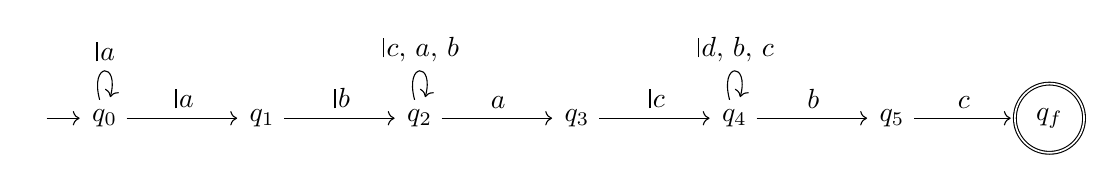
\begin{tikzpicture}[shorten >=1pt,node distance=2cm, auto, initial text={}]
              \node[initial] (q0) {$q_0$};
              \node (q1) [right of=q0] {$q_1$};
              \node (q2) [right of=q1] {$q_2$};
              \node (q3) [right of=q2] {$q_3$};
              \node (q4) [right of=q3] {$q_4$};
              \node (q5) [right of=q4] {$q_5$};
              \node[state, accepting] (qf) [right of=q5] {$q_f$};
              \path[->] (q0) edge[loop above] node[midway, above] {$\newletter{a}$} ();
              \path[->] (q2) edge[loop above] node[midway, above] {$\newletter{c},\, a,\, b$} ();
              \path[->] (q4) edge[loop above] node[midway, above] {$\newletter{d},\, b,\, c$} ();
              \draw[->] (q0) -- (q1) node[midway, above] {$\newletter{a}$};
              \draw[->] (q1) -- (q2) node[midway, above] {$\newletter{b}$};
              \draw[->] (q2) -- (q3) node[midway, above] {$a$};
              \draw[->] (q3) -- (q4) node[midway, above] {$\newletter{c}$};
              \draw[->] (q4) -- (q5) node[midway, above] {$b$};
              \draw[->] (q5) -- (qf) node[midway, above] {$c$};
          \end{tikzpicture}
      \end{center}
Its literal language $L_0\seq \barAs_0$ is given by the regular expression $\newletter a \newletter a \newletter b (\newletter c + a + b)^* a\newletter c(\newletter d + b + c)^*bc$, and its bar language $L\seq \barAs$ consists of all bar strings $\alpha$-equivalent to some bar string in $L_0$. The bar language $L$ can be learned using our algorithm in \Cref{sec:learningRNNA} (like every bar language accepted by some bar NFA), and by learning $L$ we can also infer its corresponding data language under local freshness semantics, which is given by
      \[ D(L) = \setw{{u}ab{v}ac{w}bc}{{u}, {v}, {w} \in \Ats,\ 
          a \neq b, b \neq c \in \names}. \]
This data language is not accepted by any deterministic nominal/register automaton, hence existing learning algorithms for such automata~\cite{DBLP:conf/tacas/DierlFHJST24,CasselHJS16,CEGAR12,mssks17} are not able to learn it.
It is also not \emph{residual} in the sense of Moerman and Sammartino~\cite{ms22}, so that their algorithm $\nu$\NLstar for learning non-deterministic nominal automata (which only guarantees termination for residual data languages) does not apply; see appendix. On the other hand, there exist data languages accepted by deterministic nominal automata that do not allow \emph{name-dropping}~\cite{skmw17}, or residual non-deterministic nominal automata that require \emph{guessing}~\cite[Sec.~3]{ms22}, and hence are not expressible by bar NFAs. This means that our learning algorithm applies to classes of data languages orthogonal to the classes captured by previous algorithms.
    \end{expl}

We conclude this section with the important observation that $\alpha$-renaming is computable at the level of bar automata.
    A bar automaton $\A$ is \emph{closed} if its literal language is closed under $\alpha$-equivalence with respect to the
    finite alphabet $\barNames_0$, that is, 
$L_0(\A) = L_\alpha(\A) \restriction \barNames_0$. 
Closure can always be achieved, at the price of an exponential blowup of the number of states w.r.t. the alphabet size:

    \begin{prop}\label{prop:barautclosure}
      For every bar automaton over $\barNames_0$ with $n$ states, there
      exists a closed bar automaton over $\barNames_0$ with $\mathcal{O}(n\cdot 2^{\card{\barNamess_0}\cdot (\log{\card{\barNamess_0}} + 1)})$ states accepting the same bar language.
    \end{prop}
This is essentially a consequence of the proof of \Cref{thm:bar-vs-rnna}: converting a bar automaton into an equivalent RNNA/Büchi RNNA/RNTA and back yields a closed bar automaton.

\begin{corollary}\label{cor:restr-regular}
For every bar language $L$ accepted by some bar automaton over $\barNames_0$, the language $L\restriction \barNames_0$ is regular.
\end{corollary}
This result is the key to our approach to learning bar languages, as it enables a reduction to learning corresponding regular languages. To achieve this, we need to bridge the gap between literal and bar languages, which requires the algorithmic handling of $\alpha$-equivalence.



    \section{Checking \texorpdfstring{$\boldsymbol{\alpha}$}{$\alpha$}-Equivalence}\label{sec:checkingAlphaEquiv}

At the heart of our learning algorithms for bar automata presented in \Cref{sec:learningRNNA}, and an essential requirement for their effective implementation, is a method to check finite bar strings, ultimately periodic bar strings and bar trees for $\alpha$-equivalence. In the following we develop a suitable version of \emph{De Bruijn levels}~\cite{db72}, originally introduced as a canonical representation of $\lambda$-terms. In this way, $\alpha$-equivalence reduces to syntactic equality.
    
    \mypar{Finite Bar Strings} In the case of bar strings, the idea of De Bruijn levels is to replace all bound occurrences of some name, as well as the preceding occurrence of the bar letter creating the binding, with a suitable natural number, while leaving free names as they are. This yields a canonical representation of bar strings up to $\alpha$-equivalence.

    \begin{defn}[De Bruijn Normal Form]
        Given a bar string $w = \alpha_1 \cdots \alpha_n \in \barAs$, its \emph{De Bruijn normal form} $\nf(w) = \beta_1 \cdots \beta_n \in (\names + \Nat)^\ast$ is a word of the same length as $w$ over the alphabet $\names + \Nat$, with $\beta_i$ defined inductively as follows:
        \begin{enumerate}
            \item $\beta_i = \alpha_i$ if $\alpha_i\in \names$ and $\alpha_i$ is not preceded by any occurrence of $\newletter{\alpha_i}$ in $w$;
            \item $\beta_i = k$ if $\alpha_i \in \names$ and $\beta_j = k$ where $j = \max\setw{j < i}{\alpha_j = \newletter{\alpha_i}}$;
            \item $\beta_i = k + 1$ if $\alpha_i$ is a bar name and $\alpha_1 \cdots \alpha_{i - 1}$ contains $k$ bar names.
        \end{enumerate}
    \end{defn}
    \begin{expl}
The $\alpha$-equivalent bar strings $w = \newletter{a}c\newletter{b}b\newletter{a}a$ and $w' = \newletter{d}c\newletter{a}a\newletter{a}a$ have the same normal form, namely $\nf(w) = 1c2233 = \nf(w')$.
    \end{expl}

    The normal form $\nf(w)$ can be computed from $w$ letter by letter in polynomial time and linear-logarithmic space
    (for representing natural numbers) in the length of $w$. 
    
    \begin{proposition}\label{lem:aeDBNF}
        Two finite bar strings $v, w \in \barAs$ are $\alpha$-equivalent iff $\nf(v) = \nf(w)$.
    \end{proposition}
As an immediate consequence, we have
\begin{corollary}\label{cor:alphaeq-decidable-finite-bar-strings}
The $\alpha$-equivalence of finite bar strings is decidable in polynomial time.
\end{corollary}
Indeed, to decide whether two given bar strings $v,w\in \barAs$ are $\alpha$-equivalent, it suffices to compute their normal forms $\nf(v)$ and $\nf(w)$ and check for syntactic equality.
      

      \mypar{Infinite Bar Strings} De Bruijn normal forms for infinite bar strings could be defined in the same way as for finite bar strings. However, this normal form does not preserve ultimate periodicity (for instance, $(\newletter aa)^\omega$ has the normal form $11 22 33\cdots$). A modified normal form that does preserve it, is invariant under $\alpha$-renaming, and the representation of ultimately periodic bar strings via pairs of finite bar strings seems hard to achieve.

Nonetheless, we can check ultimately periodic bar strings for $\alpha$-equivalence by reducing to the finite case. Intuitively, given $u_1v_1^\omega$ and $u_2v_2^\omega$, since $v_1$ and $v_2$ are repeated
    infinitely often, plain names in $v_i$ are either free,
    refer back to $u_i$ or to the directly preceeding repetition of~$v_i$. This observation leads to the
    following proposition:
    \begin{proposition}\label{lem:aeinfbar}
      Two ultimately periodic bar strings $u_iv_i^\omega$ $(i=1,2)$ with $\abs{u_1} = \abs{u_2}$ are
      $\alpha$-equivalent iff their prefixes $p_i = u_i v_i^{2\ell_i}$ are $\alpha$-equivalent, where
      $\ell_1 = \abs{v_2}$ and $\ell_2 = \abs{v_1}$.
    \end{proposition}
      \noindent
      The exponents $2\ell_i$ make sure that~(a) $p_1$ and $p_2$ have the same length, (b) for every pair of positions $i_1$ in $v_1$ and $i_2$ in $v_2$, there is a position $j$ in $p_1$ and $p_2$ where the letters at $i_1$ and $i_2$ `meet', and (c) that position $j$ can be chosen such that there is a full copy of $v_i$ in $p_i$ preceeding it. Note that~(a) and~(b) would already be achieved by taking just $\ell_i$ as the exponent, and the factor $2$ then achieves~(c) while maintaining~(a) and~(b).

\begin{corollary}
The $\alpha$-equivalence of ultimately periodic bar strings (represented as pairs of finite words) is decidable in polynomial time.
\end{corollary}


    \mypar{Bar Trees} For the case of bar trees, the De Bruijn
    level notation can be reduced to that for bar strings: the normal form of a bar tree is simply given by the bar string normal form
computed for every individual branch.
    \begin{defn}
        \begin{enumerate}
            \item Given the finite signature $\Sigma$, a \emph{De Bruijn $\Sigma$-tree} is a tree over the signature $(\At+\N)\times \Sigma$ with symbols $\nicefrac{\alpha.f}{n}$ and $\nicefrac{k.f}{n}$ for $\alpha\in\barNames$, $k\in \Nat$ and $\nicefrac{f}{n}\in \Sigma$. 
            \item Given a bar $\Sigma$-tree $t \in \bartree(\Sigma)$, its \emph{De Bruijn normal form} $\nf(t)$
                is a De Bruijn $\Sigma$-tree of the same shape as $t$. For every node $x$ of $t$ with label $\alpha.f$, the corresponding node of $\nf(t)$ has the label $\beta.f$ with $\beta\in \barNames+\N$ determined as follows: let $\alpha_1.f_1,\cdots,\alpha_n.f_n,\alpha.f$ be the sequence of node labels occurring on the path from the root of $t$ to $x$, and take $\beta$ to be the last letter of the bar string normal form $\nf(\alpha_1\cdots \alpha_n\alpha)\in (\barNames+\N)^*$.
        \end{enumerate}
    \end{defn}

    It is readily verified that the computation of the Bruijn normal form can be performed in
    polynomial time in the number of nodes of the given tree. Just like in the case of bar strings, normal forms capture $\alpha$-equivalence:


  

    \begin{proposition}\label{lem:aeTrees}
        Two bar trees $s, t \in \tree_\names(\Sigma)$ are $\alpha$-equivalent iff $\nf(s) = \nf(t)$.
    \end{proposition}
Therefore, we conclude with
\begin{corollary}\label{cor:alphaeq-decidable-finite-bar-trees}
The $\alpha$-equivalence of bar trees is decidable in polynomial time.
\end{corollary}


    \section{Learning Bar Languages}\label{sec:learningRNNA}
With the technical preparation of the previous sections at hand, we present the main contribution of our paper: a learning algorithm for bar languages.  
\begin{notation}
In the following, we fix an \emph{unknown} bar word/$\omega$-/tree language $L_\teach$ recognizable by some bar word/Büchi/tree automaton with finite alphabet $\barNames_0$.\footnote{In the tree case, this means a language/automaton over the signature $\barNames_0\times \Sigma$ for a finite signature $\Sigma$.}
\end{notation}
Our learning algorithm follows Angluin's MAT framework (\Cref{sec:active-learning}), that is, it describes the strategy of a \emph{learner} $\learn_\alpha$ that interacts with a \emph{teacher} $\teach$ in order to infer a bar automaton over $\barNames_0$ accepting $L_\teach$.
As usual, $\learn_\alpha$ can direct membership and equivalence queries to \teach, which in the
present setting take the following form:
    \begin{description}
        \item[Membership Queries $(\textsf{MQ}_\alpha)$:]
            Given a finite bar string/ultimately periodic bar string/bar tree $w\in \barAs/\barAw/\bartree(\Sigma)$, is $w \in L_\teach$?
        \item[Equivalence Queries $(\textsf{EQ}_\alpha)$:]
            Given a bar automaton $\H$, is $L_\alpha(\H)=L_\teach$? If not,
            then \teach provides a counterexample, that is, a finite bar string/ultimately periodic
            bar string/bar tree $w_\teach\in \barAs/\barAw/\bartree(\Sigma)$ in the symmetric difference $L_\alpha(\H)\oplus L_\teach$.
    \end{description}
 We assume that $\learn_\alpha$ is aware of the finite alphabet $\barNames_0$ of the unknown bar automaton. Interpreting bar automata as register automata (\Cref{sec:bar-automata}), this boils down to the number of registers being known. In \Cref{sec:alphabet}, we describe how to learn $L_\teach$ without this information. 

The learner $\learn_\alpha$ consists of two components, depicted in \Cref{fig:talearner}. 
    \begin{figure*}[t]
        \centering
        \begin{tikzpicture}[%
    every node/.style={align=center}]

    \node[anchor=north west, draw=black, thick, minimum height=0.05\linewidth, minimum width=0.65\linewidth, rounded corners]
        (L) at (0,0) {\textsf{L}};

    \node[anchor=north west, draw=black, thick, minimum height=0.29\linewidth, minimum width=0.65\linewidth, rounded corners]
        (TA) at (0,-0.1\linewidth) {};

    \node[draw, diamond, aspect=2, scale=0.65] (D2) at (0.21\linewidth,-0.275\linewidth) {$\exists\,w'\alphaequiv w:$\\ $w'\in L_0(\H)$?};
    \node[anchor=south west,text=lipicsGray] at ($(D2.north east) + (-1pt,-1pt)$) {\bfseries\textsf{2}};
    
    \node[anchor=south west] at ($(D2.south west) + (-1.05,-0.5)$) {\textsf{TA}};
    
    \node[draw, trapezium, trapezium left angle=70, trapezium right angle=110,
            scale=0.65] (COR) at ($(D2.east) + (2.25,0)$) {Compute $w \alphaequiv w_\teach$\\over $\barNames_0$};
            
    \node[anchor=north west,text=lipicsGray] at ($(COR.south east) + (14pt,1pt)$) {\bfseries\textsf{1}};
    

    \node[anchor=north, inner sep=0] (GL) at ($(TA.south) + (0,-0.1)$) {$\learn_\alpha$};
    \node[fit=(TA)(L)(GL), draw=black, thick, rounded corners, dotted] (BOXGENLEARN) {};

    \node[anchor=west, draw=black, thick, minimum height=0.05\linewidth, minimum width=0.2\linewidth, rounded corners] (T)
        at (0.75\linewidth, -0.21\linewidth) {\textsf{T}};

    \draw[rounded corners, -latex, ultra thick] ($(L.south east) + (-0.05\linewidth,0)$)
    -- node[scale=0.65, pos=0.2, right] {(\textsf{MQ})} node[scale=0.65, pos=0.4, right] {$w$} ++(0,-0.07\linewidth) 
    -| node[scale=0.65, pos=0.6, right] {($\textsf{MQ}_\alpha$)}
    node[scale=0.65,pos=0.75,right] {$w$}($(T.north west) + (0.1\linewidth,0)$);
    \draw[rounded corners, dashed, -latex, very thick] 
        let \p1 = (L.south), \p2 = ($(T.north) + (0,0.045\linewidth)$) in
        ($(T.north) + (-0.025\linewidth,0)$) -- ++(0,0.045\linewidth) -- node[pos=0.165, below, scale=0.65] {\textsc{Yes}/\textsc{No}} (\x1,\y2)
        -- (L.south);

    \draw[rounded corners, -latex, ultra thick]
        ($(L.south west) + (0.095\linewidth, 0)$) |-
        node[pos=0.045, scale=0.65, right] {(\textsf{EQ})}
        node[pos=0.1, scale=0.65, right] {$\H$}
        node[pos=0.96,above,scale=0.65] {($\textsf{EQ}_\alpha$)} node[pos=0.96,below,scale=0.65] {$\H$} (T.west);

    

    \draw[very thick, rounded corners, dashed] (T.south) |- 
        node[pos=0.25, right, scale=0.65] {\textsc{Yes}/$w_{\textsf{T}}$} ($(COR.east) + (3,0)$);
    \draw[very thick, rounded corners, dashed] ($(COR.east) + (3,0)$) -| ($(COR.east) + (2.5,-0.5)$);
    \draw[-latex, very thick, rounded corners, dashed] 
        let \p1 = (BOXGENLEARN.east), \p2 = ($(COR.east) + (0,-0.75)$) in ($(COR.east) + (2.5,-0.5)$) |- 
        node[pos=0.7, above, scale=0.65] {\textsc{Yes}} (\x1,\y2);
    
    \draw[-latex, very thick, rounded corners, dashed] ($(COR.east) + (3,0)$) -- node[pos=0.75, above, scale=0.65] {$w_{\textsf{T}}$} (COR.east);

    \draw[-latex, very thick, rounded corners, dashed]
        (COR.west) -- node[midway, above, scale=0.65] {$w$} (D2.east);
    
    \coordinate (AAAA) at ($(D2.west) + (-0.75,0)$);
    \coordinate (AAAB) at ($(COR.east) + (0,2)$);

    
    \draw[-latex, dashed, rounded corners, very thick]
        let \p1 = (AAAA), \p2 = (AAAB), \p3 = (L.south) in
        (D2.west) -| node[pos=0.15, above, scale=0.65] {\textsc{false}} node[pos=0.15, below, scale=0.65] {$w$}
        node[pos=0.93,right,scale=0.65] {$w$} (\x1,\y3);
    
    
    \draw[dashed, rounded corners, very thick]
        (D2.south) |- node[pos=0.175, left, scale=0.65] {\textsc{true}}
        node[pos=0.15, right, scale=0.65] {$w'$} ($(D2.south) + (-1,-0.5)$);
    
    \draw[dashed, rounded corners, very thick, -latex] 
        let \p1 = ($(D2.west) + (-1.15,0)$), \p2 = (L.south) in
        ($(D2.south) + (-1,-0.5)$) -| node[pos=0.95,left,scale=0.65] {$w'$} (\x1,\y2);
\end{tikzpicture}%

        \caption{\label{fig:talearner}Learner $\learn_\alpha$ with internal learner \learn, teaching assistant \tass and  teacher \teach.}
    \end{figure*}
The first component is an \emph{arbitrary} MAT-based learner \learn for standard regular word/$\omega$-/tree languages over $\barNames_0$ that infers a finite automaton/Büchi automaton/tree automaton using a finite number of membership queries $(\textsf{MQ})$ and equivalence queries $(\textsf{EQ})$.  The learner \learn may, for instance, execute any of the learning algorithms discussed in \Cref{sec:active-learning}. The precise choice of \learn's algorithm affects the query complexity of $\learn_\alpha$, but not its correctness and termination.

The second component of $\learn_\alpha$ is a \emph{teaching assistant} (\tass) that internally interacts with \learn and externally interacts with the teacher \teach. In the interaction with \learn, the \tass emulates a teacher for the language $L_\teach \restriction \barNames_0$; recall from \Cref{cor:restr-regular} that this is a regular language. To achieve this, the \tass turns each query $(\textsf{MQ})$ and $(\textsf{EQ})$ of \learn into a corresponding query $(\textsf{MQ}_\alpha)$ and $(\textsf{EQ}_\alpha)$ for the teacher \teach. Subsequently, the \tass translates \teach's answer back to a form that \learn can process.  
In more detail, the \tass proceeds as shown in \Cref{fig:talearner}:
\begin{itemize}
\item A membership query ($\textsf{MQ}$) by $\learn$ (given by a bar string/ultimately periodic bar string/bar tree $w\in \barNames_0^*/\barNames_0^\omega/\bartree[\barNamess_0](\Sigma)$) and its answer are relayed
    unchanged between \learn and \teach.
\item For an equivalence query ($\textsf{EQ}$) by \learn with hypothesis $\H$ (a bar word
  automaton/bar Büchi automaton/bar tree automaton over $\barNames_0$), the query itself is
  relayed unchanged to \teach. If~$\H$ is correct (i.e.~$L_\alpha(\H)=L_\teach$), then the learner $\learn_\alpha$ successfully terminates. Otherwise \teach
    returns a counterexample $w_\teach \in \barAs/\barAw/\bartree(\Sigma)$ in the symmetric difference $L_\alpha(\H)\oplus L_\teach$. 
\item The \tass cannot simply relay the counterexample $w_\teach$ to the internal learner \learn because the latter expects a counterexample over the finite alphabet $\barNames_0$. Therefore, $w_\teach$ needs to be suitably processed. First, the \tass picks any bar string/ultimately periodic bar string/bar tree $w$ over the finite alphabet $\barNames_0$ that is $\alpha$-equivalent to $w_\teach$ (step $\mathsf{1}$ in \Cref{fig:talearner}). Note that such $w$ always exists because the bar languages $L_\alpha(\H)$ and $L_\teach$ are both accepted by bar automata over $\barNames_0$. Second, $w$ is chosen to be in the literal language of the hypothesis~$\H$ if possible (step~$\mathsf{2}$ in \Cref{fig:talearner}), and then returned to \learn. 
\end{itemize}

We will explain below how $w$ and $w'$ in steps $\mathsf{1}$ and $\mathsf{2}$ can be
effectively computed by the \tass. First, let us prove that the algorithm of \Cref{fig:talearner} indeed learns a bar automaton for $L_\teach$:
    

    \begin{theorem}[Correctness]\label{lem:correctEverything}%
      Suppose that the internal learner
      \learn needs ${M(L_\teach\restriction \barNames_0)}$ membership and $E(L_\teach\restriction \barNames_0)$ equivalence queries to learn a finite automaton/Büchi automaton/tree automaton for the regular language
      $L_\teach \restriction \barNames_0$. Then $\learn_\alpha$ learns a
      bar automaton for $L_\teach$ with at most $M(L_\teach \restriction \barNames_0)$ membership and $E(L_\teach\restriction \barNames_0)$ equivalence
      queries.
    \end{theorem}
    \begin{proof}
Clearly, if the learner $\learn_\alpha$ terminates, then it has inferred a correct bar automaton for the unknown bar language $L_\teach$. Thus, we only need to establish $\learn_\alpha$'s query complexity. As indicated above, the key observation is that all answers the internal learner \learn receives from the \tass correspond to answers of a teacher for the regular language $L_\teach\restriction \barNames_0$; that is,
\begin{enumerate}
\item\label{claim-1} If \learn asks a membership query $w\in
  \barAs_0/\barAw_0/\bartree[\barNamess_0](\Sigma)$, %
  the \tass answers `Yes' iff $w\in L_\teach\restriction \barNames_0$.
\item\label{claim-2} If \learn asks an equivalence query with hypothesis $\H$ (a bar automaton
  over $\barNames_0$), then the answer of the \tass (if any) is an element of the symmetric difference $L_0(\H) \oplus (L_\teach\restriction \barNames_0)$. 
\end{enumerate}
Note that the \tass might not answer an equivalence query by \learn at all: if $\H$ satisfies
$L_\alpha(\H)=L_\teach$, then $\learn_\alpha$ successfully terminates without running $\learn$
to completion. The claimed complexity bound for $\learn_\alpha$ is then immediate: Since
$\learn_\alpha$ simply forwards each of $\learn$'s membership and equivalence queries to
\teach, the total number of $\learn_\alpha$'s queries is at most $M(L_\teach\restriction
\barNames_0)$ and $E(L_\teach\restriction \barNames_0)$, respectively. It remains to prove the
statements in \labelcref{claim-1,claim-2}.

\smallskip\noindent
\emph{Proof of \cref{claim-1}.} Since a membership query $w$ by \learn is a bar string/ultimately periodic bar string/bar tree over $\barNames_0$, we have $w\in L_\teach\restriction \barNames_0$ iff $w\in L_\teach$. Therefore \teach's answer to the query `$w\in L_\teach$?', which the \tass forwards to \learn, is also a correct answer for \learn's query `$w\in L_\teach\restriction \barNames_0$?'.      

\smallskip\noindent \emph{Proof of \cref{claim-2}}. Suppose that $\H$ is an incorrect hypothesis for $L_\teach$, that is, $L_\alpha(\H)\neq L_\teach$, so that \teach returns an element $w_\teach$ of the symmetric difference $L_\alpha(\H) \oplus L_\teach$ to $\learn_\alpha$. Let $w\alphaequiv w_\teach$ be the $\alpha$-equivalent bar string/ultimately periodic bar string/bar tree over $\barNames_0$ chosen by the~\tass in step $\mathsf{1}$. We consider the following two cases:
\begin{itemize}
\item Case 1: $w_\teach\in L_\teach\setminus L_\alpha(\H)$. Then $w\in L_\teach\setminus L_\alpha(\H)$ because both $L_\teach$ and $L_\alpha(\H)$ and hence $L_\teach\setminus L_\alpha(\H)$ are closed under $\alpha$-equivalence. Since $w\not\in L_\alpha(\H)$, there exists no $w'\in L_0(\H)$ such that $w'\alphaequiv w$, so the \tass returns $w$ to \learn after step $\mathsf{2}$. Then $w\in (L_\teach\restriction \barNames_0)\setminus L_0(\H)$, in particular $w\in  L_0(\H)\oplus (L_\teach\restriction \barNames_0)$ as claimed.
\item Case 2: $w_\teach\in L_\alpha(\H)\setminus L_\teach$. Then $w\in L_\alpha(\H)\setminus L_\teach$, analogous to Case 1. Since $w\in L_\alpha(\H)$, there exists $w'\in L_0(\H)$ such that $w'\alphaequiv w$. The \tass picks one such $w'$ in step $\mathsf{2}$ and returns it to \learn. Note that $w'\not\in L_\teach$ because $w\not\in L_\teach$ and $L_\teach$ is closed under $\alpha$-equivalence. Therefore $w'\in L_0(\H)\setminus (L_\teach\restriction \barNames_0)$, whence $w'\in L_0(\H)\oplus (L_\teach\restriction \barNames_0)$ as claimed.\qedhere
\end{itemize}   



    \end{proof}
It remains to address the implementation of steps $\mathsf{1}$ and $\mathsf{2}$ in \Cref{fig:talearner} by the $\tass$.
    \mypar{Computing representatives over $\boldsymbol{\barNames_0}$ (step
      $\boldsymbol{\mathsf{1}}$)} To compute an $\alpha$-equivalent word $w \alphaequiv w_\teach$ over the finite
    alphabet $\barNames_0$, the \tass proceeds as follows.
    
    For a finite bar string/bar tree $w_\teach$ over $\barNames$, non-derministically guess a finite bar string/bar tree $w$ over the finite
    alphabet $\barNames_0$ of equal length/shape, and then check $w_\teach$ and $w$ for $\alpha$-equivalence by computing the De Bruijn normal forms 
    (\Cref{cor:alphaeq-decidable-finite-bar-strings,cor:alphaeq-decidable-finite-bar-trees}). This computation requires non-deterministic
    polynomial time with respect to the size of $w_\teach$.

  For the case of an ultimately periodic infinite bar string $w_\teach = uv^\omega$, a normal
  form is not available (\Cref{sec:checkingAlphaEquiv}), so we use an alternative (and less efficient) approach for computing~$w$.
Let $\barNames_1=\set{\alpha\in \barNames\mid \text{$\alpha$ occurs in $w_\teach$}}$. First,
build a Büchi automaton with finite alphabet $\barNames_0\cup \barNames_1$ that accepts only
$w_\teach$ (with $\mathcal{O}(\card{uv})$ states). Construct its closure, that is, a Büchi automaton accepting all infinite bar strings $w\alphaequiv w_\teach$ over $\barNames_0 \cup \barNames_1$, which needs $\mathcal{O}(\card{uv} \cdot 2^{(\card{\barNamess_0}+\card{\barNamess_1})\cdot (\log(\card{\barNamess_0}+\card{\barNamess_1}) + 1)})$ states (\Cref{prop:barautclosure}), and restrict its input alphabet to $\barNames_0$ by removing all $\barNames_1\setminus \barNames_0$-transitions. The resulting Büchi automaton $\A$ accepts the language $L_0(\A)=\setw{w \in \barAw_0}{w \alphaequiv w_\teach}$. Thus, it remains to look for some ultimately periodic word $w$ in $L_0(\A)$. This is standard: perform a depth-first search to detect a cycle in $\A$ (with label $v_1$) that contains a final state and is reachable from the initial state (via some path with label $u_1$). Then $w=u_1v_1^\omega$ is an ultimately periodic bar string contained in $L_0(\A)$. Overall, this algorithm uses space linear in $\card{uv}$ and exponential in
    $\card{\barNames_0}$ and $\card{\barNames_1}$.   

    \mypar{Checking membership up to $\boldsymbol{\alpha}$-equivalence (step $\boldsymbol{\mathsf{2}}$)} Lastly, we explain how to decide, for $w$ computed in step $\mathsf{1}$, whether there exists an $\alpha$-equivalent $w'\in L_0(\H)$.

    For the case of finite bar strings/trees, non-deterministically guess a bar string/tree
    $w'$ of the same length/shape as $w$ and verify that $w'\alphaequiv w$ via the Bruijn normal form as before. Moreover, verify that the bar automaton $\H$ literally accepts $w'$ by guessing an accepting run. This requires
    non-deterministic polynomial time with respect to $\card{w}$.

    Again, a different approach is needed for ultimately periodic infinite bar strings. Take the Büchi automaton $\A$  constructed above with $\mathcal{O}(\card{uv} \cdot 2^{(\card{\barNamess_0}+\card{\barNamess_1})\cdot (\log(\card{\barNamess_0}+\card{\barNamess_1}) + 1)})$ states and accepting $L_0(\A)=\setw{w \in \barAw_0}{w \alphaequiv w_\teach}$, and check the intersection $L_0(\A) \cap L_0(\H)$ non-emptiness. This is achieved by searching for an ultimately periodic word in \mbox{$L_0(\A)\cap L_0(\H)$}, where a Büchi automaton for the intersection can be formed via a standard product construction. In total, this requires space linear in the length of the counterexample and the
    number of states of the hypothesis, and again exponential in 
    $\card{\barNames_0}$ and $\card{\barNames_1}$.   






    \section{Handling Unknown Input Alphabets} \label{sec:alphabet}

    Finally, we discuss how to lift the previous requirement of having a known finite
    alphabet generating the unknown bar language $L_\teach$. The idea is to run the learner $L_\alpha$ with \emph{any} finite alphabet $\barNames_0\seq \barNames$. In case $L_\alpha$ gets stuck, it knows that the present alphabet is too small and reboots the learning process with a suitably extended alphabet. Details are as follows.

Initially, $L_\alpha$ is executed (running the learning algorithm of \Cref{fig:talearner}) with
the trivial alphabet $\barNames_0=\emptyset$. If a correct hypothesis is found, then $L_\alpha$
successfully terminates. If \teach delivers a counterexample $w_\teach$, then it may occur in the computation of step $\mathsf{1}$ that no $w\alphaequiv w_\teach$ over $\barNames_0$ is found. In this case, $\barNames_0$ is extended to a larger finite alphabet  $\barNames_0\seq \barNames_0'\seq \barNames$ such that a representative $w$ of $w_\teach$ over $\barNames_0'$ exists; we explain below how to compute a suitable~$\barNames_0'$. Then~$L_\alpha$ restarts with the new alphabet $\barNames_0'$. This process of alphabet extension and restarting~$L_\alpha$ is repeated each time step $\mathsf{1}$ gets stuck. At some stage, the current alphabet is large enough to generate the unknown bar language $L_\teach$, and then $L_\alpha$ successfully runs to completion.

It remains to explain how to extend the current $\barNames_0$ to a larger $\barNames_0'$. In the case of finite bar strings/trees, compute the De Bruijn normal form of $w_\teach$ and choose the extension $\barNames_0\seq \barNames_0'$ to be a smallest possible alphabet such that some $w\alphaequiv w_\teach$ over $\barNames_0'$ exists. The number of bar and plain letters that need to be added to $\barNames_0$ can be read off the normal form.

 In the case of infinite bar strings, construct a Büchi automaton accepting the closure of the ultimately periodic bar string $w_\teach$ with respect to the alphabet $\barNames_0\cup \barNames_1$, where $\barNames_1$ is the set of letters appearing in $w_\teach$ (cf.\ \Cref{sec:learningRNNA}), and then search for a smallest subalphabet $\barNames_0\seq\barNames_0'\seq (\barNames_0\cup\barNames_1)$%
 such that this closure contains some ultimately periodic bar string over~$\barNames_0'$. Note that $\barNames_0'$ necessarily contains all free names of $w_\teach$.

    This process of iterated alphabet extension approximates a fitting alphabet from below, ending at a smallest possible $\barNames_0$ that generates $L_\teach$, that is, such that $L_\teach$ is the closure of $L_\teach\restriction \barNames_0$ under $\alpha$-equivalence. To estimate the query complexity of the above algorithm, let us introduce some notation. We write $M(L)$ and $E(L)$ for the number of membership and equivalence queries required by the internal learner \learn to learn a regular language $L$. Moreover, for $k\in \Nat$ we put $M_k = \max \set{M(L_\teach \restriction \barNames_0) \mid \barNames_0\seq \barNames,\, \card{\barNames_0}=k}$; similarly for $E_k$.
\begin{theorem}[Correctness]
Let $n$ be the least cardinality of any finite alphabet $\barNames_0\seq \barNames$ generating $L_\teach$. Then the above extended learning algorithm infers a bar automaton for $L_\teach$ with at most $\sum_{k = 0}^n M_k$ membership queries and $\sum_{k = 0}^n E_k$ 
equivalence queries.
    \end{theorem}

\begin{proof}
Let $n_i$ be the size of the finite alphabet used in the $i$th iteration of $L_\alpha$. Since the alphabet grows in every iteration, we have $0=n_0<\ldots<n_k=n$, where $k+1$ is the total number of iterations. The number of membership queries in the $i$th iteration is at most~$M_{n_i}$, and so the total number of membership queries is at most $\sum_{i=0}^k M_{n_i} \leq \sum_{i=0}^n M_i$. The same reasoning applies to equivalence queries.
\end{proof}

    \begin{rem}
        An alternative to restarting the learner $L_\alpha$ (and hence the internal learner \learn) each time the alphabet  grows is to use a learner $\learn$ that can handle \emph{dynamically growing input alphabets}, that is,
        can process counterexamples that are not over the current finite alphabet~\cite{ihs13}. In requiring such types
        of learners beforehand, the \tass procedure presents counterexamples to \learn using the minimal number of
        additional letters. The learner \learn then
        needs to handle the \emph{grown} alphabet internally and proceed. This method potentially saves queries compared to a  restart but restricts the class of
        possible learners significantly. To the best of our knowledge, learners for dynamically growing alphabets have only been studied in the case of deterministic automata over finite words.
    \end{rem}

    \section{Conclusion and Future Work}\label{sec:concl}

    We have investigated the learnability of bar word languages, bar $\omega$-languages and bar tree languages in Angluin's minimally adequate teacher (MAT) framework. For this purpose, we
    have introduced a learning algorithm $\learn_\alpha$ which relies on an arbitrary MAT-based learner for
    standard word/$\omega$-/tree languages over finite alphabets. Its query complexity is completely determined by
    the underlying learner.
    In addition, one of its key ingredients is an efficient procedure for checking
    $\alpha$-equivalence of bar strings/terms. For the latter, we have developed a suitable
    version of \emph{De Bruijn levels}~\cite{db72} reducing the problem to checking syntactic
    equality.

    There are various directions for future work. When learning bar $\omega$-languages, we 
    currently compute closures of bar automata, which is not needed in the cases of finite bar strings and trees where we instead guess a suitable De Bruijn normal form. It remains to investigate whether a guessing approach is possible in the infinite case; as a technical prerequisite, this would require a suitable normal form for ultimately periodic bar strings.

    Looking at data languages (bar languages under local
    freshness), a further question is whether we can efficently learn such languages without needing an explicit representation
    as bar automata, and in particular without needing associated membership and equivalence queries. 
	The key challenge is that the local freshness operator is not injective, so that there is no straightforward back-and-forth translation between bar and data languages. A related question arises for the
     global freshness semantics, where the operator is also not injective.
    
Another open problem is the possibility of conformance testing for bar automata, which is a common approach for implementing equivalence queries in a practical black-box learning setting (e.g.~\cite{DBLP:journals/cacm/Vaandrager17}). 
	Likewise, passive learning of bar languages is an open problem.

	 An alternative to the approach of the present paper would be to develop learning algorithms directly
	at the level of bar automata or equivalent models such as RNNAs, instead of reducing
	them to standard learning algorithms for non-data languages. We believe that the categorical
	approaches to automata learning~\cite{us20,hkrss22} would be a good starting point. 
	



    \bibliography{refs}


\appendix
\subsection*{Appendix}
This appendix contains proof details omitted in the paper. In particular, we explain the connection between bar automata and nominal automata.

    \section{Details for~\Cref{sec:prelim}}\label{app:EquivModels}
    
\mypar{More on Nominal Sets}
We recall additional terminology from the theory of nominal sets, which is needed for some of the proofs and constructions presented in the sequel.

    An element $x$ of a nominal set $X$ is \emph{equivariant} if it has an empty support, i.e.~$\supp(x) = \emptyset$, while a subset $X$ of a nominal set $Y$ is \emph{equivariant} if $\pi\cdot x\in X$ for all $x\in X$ and $\pi\in\Perm(\names)$.
    A map $f\colon X \to Y$ between nominal sets is \emph{equivariant} if $f(\pi \cdot x) = \pi \cdot f(x)$ for all $x \in X$ and $\pi \in \Perm(\names)$, which implies $\supp f(x) \subseteq \supp x$ for all $x \in X$.
    Similarly, a subset $X$ has \emph{support} $S$ if $\pi \cdot x \in X$ for all $x \in X$ and permutations $\pi$ such that $\pi(a) = a$ for all $a \in S$.
    $X$ is \emph{uniformly finitely supported} if $\bigcup_{x \in X} \supp(x)$ is finite, in which case $X$ is also finitely supported. A uniformly finitely supported equivariant set consists of only elements that are themselves equivariant.

    The coproduct of nominal sets $X_i$ ($i\in I$) is given by their disjoint union $\coprod_{i\in I} X_i = \setw{(i,x)}{i\in I,\, x\in X_i}$ with groups action inherited from the $X_i$, that is, $\pi\cdot (i,x)=(i,\pi\cdot x)$.

    Given a nominal set $X$, the \emph{orbit} of an element $x\in X$ is the set  $\setw{\pi\cdot x}{\pi \in \Perm(\names)}$. The orbits form a partition of $X$.
    A nominal set is \emph{orbit-finite} if it has finitely many orbits. For every finite set $S\seq\names$, an orbit-finite nominal set contains only finitely many elements supported by $S$. The \emph{degree} of an orbit-finite nominal set $X$ is  $\deg(X) = \max_{x\in X} |\supp(x)|$. 

    \begin{expl}
     The nominal set $\Ats$ has infinitely
        many orbits; its equivariant subsets $\names^n$ (words of a fixed length $n$) are orbit-finite. For instance,
        $\names\!^2$ has the two orbits $\{aa: a\in \names\}$ and $\{ab: a\neq b\in \names\}$.
        Another example of an orbit-finite nominal set is \[\names\!^{\#n} = \setw{a_1\ldots a_n}{a_i\neq a_j
        \text{ for $i\neq j$}},\]
an equivariant subset of $\names^n$ with just a single orbit.
        Both $\names^{\# n}$ and $\names^n$ have degree $n$.
    \end{expl}

    \mypar{Details for~\Cref{thm:bar-vs-rnna}}
    We prove the claim that all bar automata (bar NFAs/bar Büchi automata/bar NFTAs) have an equi-expressive
    nominal model in more detail. The claim was proven for bar NFAs and regular non-deterministic nominal
    automata (RNNA) in the original paper by Schröder et al.~\cite[Corollary 5.14]{skmw17}, but for
    both bar Büchi automata~\cite[Proof of Thm.~6.2]{uhms21} as well as bar NFTAs~\cite[Proof of Thm.~6.3]{ps24}
    only one direction (nominal to bar automaton) was shown. We begin by recalling basic definitions for
    both Büchi RNNAs and regular nominal tree automata (RNTA), and then show that every bar automaton has
    a corresponding nominal automaton accepting the same bar language.

    \subparagraph*{Büchi Automata}

    First, we recall the necessary nominal automata from~\cite{skmw17,uhms21,ps24}:
    \begin{defn}[RNNA~\cite{skmw17} and Büchi RNNA~\cite{uhms21}]
      \begin{enumerate}
        \item An \emph{RNNA} $A=\maketuple{Q, R, q_0, F}$ is given by an orbit-finite
          nominal set $Q$ of \emph{states}, an equivariant relation
          $R\seq Q\times \barA \times Q$ specifying \emph{transitions}, an \emph{initial state} $q_0 \in Q$
          and an equivariant set $F\seq Q$ of \emph{final states}. We write $q\xto{\sigma}q'$ if
          $(q,\sigma,q')\in R$. The transitions are subject to two conditions:
          \begin{enumerate}
            \item \emph{$\alpha$-invariance}: if $q\xto{\scriptnew a}q'$ and
              $\braket{a} q'=\braket{b} q''$, then $q\xto{\scriptnew b}q''$.
            \item \emph{Finite branching up to $\alpha$-invariance:} For every $q\in Q$ the sets
              $\setw{(a,q')}{q\xto{a}q'}$ and $\setw{\braket{a} q'}{q\xto{\scriptnew a} q'}$
              are finite (equivalently, uniformly finitely supported).
          \end{enumerate}
        \item A \emph{Büchi RNNA} is an RNNA $A = \maketuple{Q, R, q_0, F}$ accepting infinite bar strings
          as follows: Given $w = \sigma_1\sigma_2\cdots \in \barAw$ and a state $q \in Q$, a run for $w$
          from $q$ is an infinite sequence of transitions $q\xto{\sigma_1}q_1\xto{\sigma_2}\cdots$.
          The run is \emph{accepting} if $q_n$ is final for infinitely many $n \in \Nat$. The state $q$
          \emph{accepts} $w$ if there is an accepting run for $w$ from $q$, and $A$ \emph{accepts} $w$ if
          its initial state $q_0$ does. The \emph{literal ($\omega$-)language} $L_0(A)$ is defined by all infinite bar
          strings accepted by $A$, while its \emph{bar ($\omega$-)language} $L_\alpha(A) = \setw{w'\in \barAw}{\exists
          w \in L_0(A): w' \alphaequiv w}$ is the closure of $L_0(A)$.
      \end{enumerate}
    \end{defn}

    The idea of the constructions below is rather simple: We add \emph{registers} to each state of the bar automaton
    over $\barNames_0$, namely one for every plain name $a_i \in \barNames_0 \cap \names$ of the alphabet.
    We then consider the $a_i$-transitions in the bar automaton as a \enquote{placeholder} for the value stored
    in the corresponding register.
    Bar transitions \emph{can} but do not need to store names and are extended with respect to $\alpha$-equivalence.
    The resulting nominal state set will be one of all partial injective maps, i.e.~partial register assignments.
    In more detail:

    \begin{defn}\label{defn:dollar}
      For $n\in\Nat$, we write $\mathbf{n}=\{1,\dots,n\}$. We denote by
      $\parnom{n}$ the nominal set of all \emph{partial injective maps}
      from $\mathbf{n}$ to $\names$, with the pointwise group action.  The
      support of~$r$ is $\setw{r(x)}{x \in \dom(r)}$, where $\dom(r)$ is
      the \emph{domain} of $r$, i.e.~the set of all $x \in \mathbf{n}$ for
      which $r(x)$ is defined. The nominal set
      $\parnom{n}$ has $2^{n}$ orbits, one for each possible
      domain. A partial injective map
      $\overline{r} \in \parnom{n}$ \emph{extends} $r \in \parnom{n}$, denoted
      $r \leqslant \overline{r}$, if
      $\dom(r) \seq \dom(\overline{r})$ and~$r$ and~$\overline{r}$
      coincide on $\dom(r)$, that is, $r(x) = \overline{r}(x)$ for all
      $x \in \dom(r)$.  Given $A \seq \supp(r)$, we write $\restr{r}{A}$
      for the \emph{restriction of $r$ to $A$}. Note that $r$ extends
      $\restr{r}{A}$ and that $\supp(\restr{r}{A}) = A$. 
    \end{defn}

    \begin{construction}\label{constr:Buechi}
      \sloppypar
      Given a bar Büchi automaton $A = \maketuple{Q, \barNames_0,\!\!\!\to\!\!, q_0, F}$ such
      that 
      ${k := \card{\barNames_0 \cap \names}}$ and $\barNames_0 \cap \names = \set{a_1, \dots, a_k}$,
      we construct the Büchi RNNA $\barA = \maketuple{\overline{Q}, \to', \overline{q_0}, \overline{F}}$
      as follows:
      \begin{itemize}
        \item $\overline{Q} := \coprod_{q \in Q} \parnom{k}$;
        \item $\overline{q_0} = \maketuple{q_0, (i \mapsto a_i)}$;
        \item $\overline{F} := \coprod_{q \in F} \parnom{k}$; and
        \item transitions $\to'$:
        \begin{itemize}
          \item $\maketuple{q, r} \xra{b}\!'{}\, \maketuple{q', r'}$ iff
            $\exists i \leqslant k: r(i) = b \wedge q \xra{a_i} q' \wedge r' \leqslant r$;
          \item $\maketuple{q, r} \xra{\scriptnew{b}}\!'{}\, \maketuple{q', r'}$ iff
            there is an $\alpha \in \barNames_0\setminus\names$ such that: (i) $q \xra{\alpha} q'$;
            (ii) for all $i \leqslant k$ if $r'(i) = b$ then $\alpha = \newletter{a_i}$;
            (iii) for all $i \in \dom(r')$: $r'(i) = b$ or $r'(i) = r(i)$; and
            (iv) if $\alpha = \newletter{a_i}$ and $i \in \dom(r')$ hold for some $i$, then $r'(i) = b$.
        \end{itemize}
      \end{itemize}
    \end{construction}
    \begin{proposition}\label{prop:APPA}
      Let $A\!=\!\maketuple{Q, \barNames_0,\!\!\!\to\!\!, q_0,\!F}$ be a bar Büchi automaton and
      $\barA\!=\!\maketuple{\overline{Q},\!\!\!\to'\!\!, \overline{q_0}, \overline{F}}$ the Büchi RNNA
      of~\Cref{constr:Buechi}. Then, $L_\alpha(A) = L_0(\barA)$.
    \end{proposition}
    \begin{proof}
      \noindent\enquote{$\seq$}: Let $w \alphaequiv w' \in L_0(A)$ and $(q_i \xra{\alpha'_i} q_{i + 1})_{i \in \Nat}$
      be an accepting run for $w' = \alpha_0'\alpha_1'\alpha_2'\cdots \in \barAw_0$. We construct an accepting
      run for $w = \alpha_0\alpha_1\alpha_2\cdots \in \barAw$.
      We define $r_0\colon \mathbf{k} \to \names, i \mapsto a_i$ and for all $i = 1, 2, \dots$ the map
      \[ r_i\colon \mathbf{k} \to \names, j \mapsto \begin{cases} 
        \ub(\alpha_{i - 1}) & \text{, if $\alpha_{i - 1}' = \newletter{a_j}$ and $\ub(\alpha) \in \FN(\alpha_i\alpha_{i + 1}\cdots)$} \\
        r_{i - 1}(j) & \text{, if $\alpha_{i - 1} \neq \newletter{r_{i-1}(j)}$ and $r_i(j) \in \FN(\alpha_i\alpha_{i + 1}\cdots)$} \\
        \bot & \text{, otherwise.}
      \end{cases} \]
      This results in a run $(\maketuple{q_i,r_i} \xra{\alpha_i}\!'{}\, \maketuple{q_{i + 1},r_{i+1}})_{i \in \Nat}$
      for $w$. Acceptance is obvious by construction of $\barA$. Regarding validity, we see that for all $i \in \Nat\setminus\set{0}$, $r_i(j)$ is set to some $\beta \in \FN(\alpha_i\alpha_{i+1}\cdots)$ occurring
      at positions $\alpha_k$ such that $\alpha_k' = a_j$ and not defined if there is no such $\beta$.
      This is obvious from the definition of $r_i$.
      With this, we see that all $\maketuple{q_i,r_i} \xra{\alpha_i}\!'{}\, \maketuple{q_{i + 1},r_{i+1}}$ are indeed
      valid transitions in $\barA$.

      \noindent\enquote{$\qes$}: We simply prove that any accepted infinite bar string $w \in L_0(\barA)$ is
      $\alpha$-equivalent to an accepted infinite bar string of $A$.
      Let $(\maketuple{q_i, r_i} \xra{\alpha_i}\!'{}\, \maketuple{q_{i + 1}, r_{i + 1}})_{i \in \Nat}$ be an accepted
      run of $w = \alpha_0\alpha_1\alpha_2\cdots \in \barAw$ in $\barA$.
      Then every transition $\maketuple{q_i, r_i} \xra{\alpha_i}\!'{}\, \maketuple{q_{i + 1}, r_{i + 1}}$ has a
      corresponding transition $q_i \xra{\alpha_i'} q_{i + 1}$ with $\alpha_i' \in \barNames_0$ in $A$.
      The precise choice of these $\alpha_i$'s is irrelevant, i.e.~we only assume that each $\alpha_i'$ witnesses
      the existential quantifiers in the definition of the transitions $\xra{\alpha_i}\!'{}\,$. However, the mentioned
      choice is miniscule and affects only with those bar names not immediately stored in a register: Indeed, if
      $\alpha_i \in \names$, there must be some $j \leqslant k$ with $r_i(j) = \alpha_i$, thereby fixing $\alpha_i' =
      a_j$. If $\alpha_i \notin\names$ and $r_{i + 1}(j) = \ub(\alpha_i)$ holds for some $j \leqslant k$, then
      $\alpha_i' = \newletter{a_j}$ is fixed (by condition (ii)). Lastly, if $\alpha_i \notin\names$ and $\ub(\alpha_i)$
      is unequal to every $r_{i + 1}(j)$, we see that $\ub(\alpha_i)$ also does not occur freely in
      $\alpha_{i + 1}\alpha_{i + 2} \cdots$ by a direct consequence of the definition of plain transitions, thus giving
      an inconsequential choice overall.
      This run is also accepting by design. We therefore only have to show
      $\alpha$-equivalence of $w$ and $w' = \alpha_0'\alpha_1'\alpha_2'\cdots$ by definition, that is,
      $\alpha$-equivalence of the prefixes of length $n$ inductively:
      The base case ($n = 0$) obviously holds. For the induction step, assume that $w_n = \alpha_0\cdots\alpha_{n-1}
      \alphaequiv \alpha_0'\cdots\alpha_{n-1}' = w_n'$ by induction hypothesis. We show $w_{n + 1} \alphaequiv
      w'_{n + 1}$. We consider the cases where $\alpha_n \notin\names$ and $\alpha_n \in \names$: The former case
      holds trivially by definition and~\Cref{lem:aeDBNF}. For the latter case, if $\alpha_n \in \names$, that is,
      $\maketuple{q_n, r_n} \xra{\alpha_n}\!'{}\, \maketuple{q_{n + 1}, r_{n + 1}}$ and $\alpha_n = b \in \names$, there
      must be some $j \leqslant k$, such that $r_n(j) = b$ and $q_n \xra{a_j} q_{n + 1}$, as well as $r_{n + 1}
      \leqslant r_n$. Thus, $\alpha_n' = a_j$. There are now two possibilities:
      \begin{enumerate}
        \item There has been a prior $\newletter{b}$-transition with a corresponding $\newletter{a_j}$-transition.
          Then, both indices in the De Bruijn normal form (\Cref{lem:aeDBNF}) of $w_{n + 1}$ and $w'_{n + 1}$
          must be equal (namely to the index of the last such corresponding transition).
        \item There has been no prior $\newletter{b}$-transition with corresponding $\newletter{a_j}$-transitions.
          Thus, $b = a_j = r_0(j)$ and $a_j$ is free in $w_{n + 1}$. $a_j$ is then also free in $w_{n + 1}'$, since
          by condition (iv), if there had been an $\alpha'_{k} = \newletter{a_j}$ with $k < n$, the corresponding 
          $\alpha_k = \newletter{c}$ would have been stored in $r_k(j)$ and all subsequent $r_{i}(j)$'s. This
          resutls in the desired $\alpha$-equivalence.
      \end{enumerate}
      By induction, we see that $w \alphaequiv w'$ and thus also $L_\alpha(\barA) = L_\alpha(A)$.
    \end{proof}

    \begin{rem}
      Let $\barNames_0 \seq \barNames$ be a finite alphabet of size $k_0$ and ${k_1 := \card{\barNames_0 \cap \names}}$.
      Then, the Büchi RNNA of~\Cref{constr:Buechi} has a degree of
      $k_1 \leqslant k_0$ and $\card{Q} \cdot 2^{k_1}$ orbits. 
    \end{rem}
    
    \subparagraph*{Tree Automata} While the previously introduced tree automata were bottom-up, its nominal
    variant of \emph{regular non-deterministic tree automata} (\emph{RNTA}) is top-down. A bar (top-down)
    non-deterministic finite tree automaton $A = \maketuple{Q, \barNames_0, \Sigma, q_0, \Delta}$ has an
    \emph{initial state} $q_0$ instead of a set of final states and its transition relation $\Delta \seq
    Q \times \barNames_0 \times (\coprod_{\nicefrac{f}{n} \in \Sigma} Q^n)$ consists of rewrite rules
    of the form \[ q(\alpha.f(x_1, \dots, x_n)) \to \alpha.f(q_1(x_1), \dots, q_n(x_n)). \]
    A \emph{run} for a tree $t \in \bartree[\barNamess_0](\Sigma)$ from $q \in Q$ is a tree $\runtree(t)$ over the signature
    $Q \times \barNames_0 \times \Sigma$ subject to the following conditions:
    \begin{enumerate}
      \item Every node $\alpha.f(t_1, \dots, t_n)$ in $t$ corresponds to one node
        $q.\alpha.f(t_1', \dots,  t_n')$ in $\runtree(t)$ at the same position and vice versa.\label{run:cond:A}
      \item Every node $q.\alpha.f(q_1.t_1, \dots, q_n.t_n)$ in $\runtree(t)$ has a corresponding rewrite
        rule\label{run:cond:B} \[q(\alpha.f(x_1, \dots, x_n)) \to \alpha.f(q_1(x_1), \dots, q_n(x_n)) \in \Delta. \]
      \item The root node is annotated by $q$.\label{run:cond:C}
    \end{enumerate}
    A tree $t \in \bartree[\barNamess_0](\Sigma)$ is accepted by $A$ iff there is a run for $t$ from $q_0$.
    It is well-known (cf.~\cite[Thm.~8]{tata08}) that top-down and bottom-up NFTAs are expressively equivalent by
    reversing all rewrite rules, swapping final and initial states, and reducing those to a single one. 
    For the proof of equivalence to RNTA, we will only use top-down NFTA for the rest of this section.
    
    \begin{defn}[RNTA~\cite{ps24}]
      \begin{enumerate}
        \item A \emph{(top-down) RNTA} $A = \maketuple{Q, \Sigma, q_0, \Delta}$ is given by an orbit-finite
          nominal set of \emph{states}, a finite signature $\Sigma$, an \emph{initial state} $q_0 \in Q$
          and an equivariant set $\Delta$ of \emph{rewrite rules} of the form
          \[ q.(\gamma.f(x_1, \dots, x_n)) \to \gamma.f(q_1(x_1), \dots, q_n(x_n)), \]
          where $q_1, \dots, q_n, q \in Q$, $\gamma \in \barNames$, $\nicefrac{f}{n} \in \Sigma$ and the $x_i$
          are variables. The rewrite rules are subject to two conditions:
          \begin{enumerate}
            \item \emph{$\alpha$-invariance}: For $q,q_1,\dots,q_n,q_1',\dots,q_n' \in Q$, if
              $\braket{a}q_i = \braket{b}q_i'$ for all $1 \leqslant i \leqslant n$, then
              \begin{align*}
                q(\newletter{a}.f(x_1, \dots, x_n)) & \to \newletter{a}.f(q_1(x_1), \dots, q_n(x_n)) \in \Delta & \text{ implies } \\
                q(\newletter{b}.f(x_1, \dots, x_n)) & \to \newletter{b}.f(q_1'(x_1), \dots, q_n'(x_n)).
              \end{align*}
            \item \emph{Finite branching up to $\alpha$-equivalence:} For $q \in Q$ and $\nicefrac{f}{n} \in \Sigma$,
              the sets
              \begin{align*}
                \setw{\maketuple{a, q_1, \dots, q_n}}{q(a.f(x_1, \dots, x_n)) \to a.f(q_1(x_1), \dots, q_n(x_n)) \in
                \Delta} & \text{ and } \\
                \setw{\braket{a}\maketuple{q_1, \dots, q_n}}{q(\newletter{a}.f(x_1, \dots, x_n)) \to
                  \newletter{a}.f(q_1(x_1), \dots, q_n(x_n)) \in \Delta}
              \end{align*}
              are finite (equivalently, uniformly finitely supported).
          \end{enumerate}
        \item Rewrite rules in RNTAs are applied as with classical (top-down) NFTAs mentioned above.
          A state $q \in Q$ \emph{accepts} a term $t$ if there is a \emph{run} for $t$ from $q$.
          The \emph{literal (tree) language} $L_0(A)$ is defined by all terms $t \in
          \bartree(\Sigma)$ accepted by $A$, while its \emph{bar (tree) language} $L_\alpha(A) =
          \setw{t' \in \bartree(\Sigma)}{\exists t \in L_0(A): t' \alphaequiv t}$ is the closure of $L_0(A)$.
      \end{enumerate}
    \end{defn}
    
    \begin{construction}\label{constr:RNTA}
      \sloppypar
      Given a bar top-down NFTA $A = \maketuple{Q, \barNames_0, \Sigma, q_0, \Delta}$ such that
      ${k := \card{\barNames_0 \cap \names}}$ and $\barNames_0 \cap \names = \set{a_1, \dots, a_k}$,
      we construct the RNTA $\barA = \maketuple{\overline{Q}, \Sigma, \overline{q_0}, \Delta'}$
      as follows:
      \begin{itemize}
        \item $\overline{Q} := \coprod_{q \in Q} \parnom{k}$;
        \item $\overline{q_0} = \maketuple{q_0, (i \mapsto a_i)}$;
        \item $\overline{F} := \coprod_{q \in F} \parnom{k}$; and
        \item rewrite rules $\Delta'$ (for $\nicefrac{f}{n} \in \Sigma$):
        \begin{itemize}
          \item $\maketuple{q,r}(b.f(x_1, \dots, x_n)) \to b.f(\maketuple{q_1,r_1}(x_1),\dots,\maketuple{q_n,r_n}(x_n))
            \in \Delta'$ iff there is an $i \leqslant k$ such that:
            \begin{itemize}
              \item $r(i) = b$;\label{RNTA:cond:1:a}
              \item for all $j \leqslant n$: $r_j \leqslant r$; and\label{RNTA:cond:1:b}
              \item $q(a_i.f(x_1, \dots, x_n)) \to a_i.f(q_1(x_1), \dots, q_n(x_n)) \in \Delta$.\label{RNTA:cond:1:c}
            \end{itemize}
          \item $\maketuple{q,r}(\newletter{b}.f(x_1, \dots, x_n)) \to \newletter{b}.f(\maketuple{q_1,r_1}(x_1),\dots,
            \maketuple{q_n,r_n}(x_n)) \in \Delta'$ iff
            there is an $\alpha \in \barNames_0\setminus\names$ such that: 
            \begin{itemize}
              \item for all $j \leqslant n, i \leqslant k$: if $r_j(i) = b$, then $\alpha = \newletter{a_i}$;
                \label{RNTA:cond:2:a}
              \item for all $j \leqslant n, i \leqslant k$: if $\alpha = \newletter{a_i}$ and $i \in \dom(r_j)$, then
                $r_j(i) = b$; \label{RNTA:cond:2:b}
              \item for all $j \leqslant n, i \in \dom(r_j)$: $r_j(i) \in \set{b, r(i)}$; and\label{RNTA:cond:2:c}
              \item $q(\alpha.f(x_1, \dots, x_n)) \to \alpha.f(q_1(x_1),\dots,q_n(x_n)) \in \Delta$.
                \label{RNTA:cond:2:d}
            \end{itemize}
        \end{itemize}
      \end{itemize}
    \end{construction}

    \begin{proposition}
      Let $A = \maketuple{Q, \barNames_0, \Sigma, q_0, \Delta}$ be a bar (top-down) NFTA and $\barA =
      \maketuple{\overline{Q}, \Sigma, \overline{q_0}, \Delta'}$ be the RNTA of~\Cref{constr:RNTA}. Then,
      $L_\alpha(A) = L_0(\barA)$.
    \end{proposition}
    \begin{proof}
      \noindent\enquote{$\seq$}: Let $t \in L_\alpha(A)$, that is, $t \alphaequiv t' \in L_0(A)$ and $\runtree(t')$
      be the run of $t'$. We translate this run to a run for $t$ in $\barA$ by defining a recursive function
      $\trans\colon \parnom{k} \times \bartree[Q \times \barNamess_0](\Sigma) \to \bartree[\overline{Q} \times
      \barNamess](\Sigma)$ via
      \[ \trans(r, \alpha'.f(t'_1, \dots, t'_n)) = \maketuple{q, r}.(\alpha.f(\trans(r_1, t'_1), \dots, \trans(r_n, t'_n))), \]
      where $\alpha.f$ is the corresponding node to $\alpha'.f$ in $t$. The $r_i \in \parnom{k}$ are defined pointwise,
      we have
      \[ r_i\colon \mathbf{k} \to \names, j \mapsto \begin{cases}
        \ub(\alpha) & \text{, if $\alpha' = \newletter{a_j}$ and $a_j \in \FN(t_i')$} \\
        r(j) & \text{, if $\alpha \neq \newletter{r(j)}$ and $r(j) \in \FN(t_i)$} \\
        \bot & \text{, otherwise.}
      \end{cases} \]
      We readily verify that $\trans(r_0, t')$ is a run for $t$ from $\overline{q_0}$: Conditions~\ref{run:cond:A}
      and~\ref{run:cond:C} are satisfied by construction. Regarding condition~\ref{run:cond:B} for an arbitrary
      node $\maketuple{q,r}.\alpha.f(\maketuple{q_1, r_1}.t_1, \dots, \maketuple{q_n, r_n}.t_n)$ in $\trans(r_0, t')$,
      we check that there is a rewrite rule \[\maketuple{q,r}(\alpha.f(x_1, \dots, x_n)) \to \alpha.f(\maketuple{q_1, r_1}x_1, \dots, \maketuple{q_n, r_n}x_n) \in \Delta'.\]
      This is obvious for $\alpha \in \barNames\setminus\names$,
      while for $\alpha \in \names$ it follows directly from the definition of $r_0$ and all subsequent $r_i$'s.
      Thus, $t \in L_0(\barA)$.

      \noindent\enquote{$\qes$}: We show that any $t \in L_0(\barA)$ is $\alpha$-equivalent to some $t' \in L_0(A)$.
      Let $\runtree(t)$ be the run for $t$ in $\barA$, then by condition~\ref{run:cond:B} all nodes
      $\maketuple{q,r}.\alpha.f(\maketuple{q_1, r_1}.t_1, \dots, \maketuple{q_n, r_n}.t_n)$ come from rewrite rules
      $q(\alpha'.f(x_1, \dots, x_n)) \to \alpha'.f(q_1(x_1), \dots, q_n(x_n))$ in $A$. Thus, replacing any $\alpha$ in
      $t$ by the corresponding $\alpha'$ results in some $t' \in L_0(A)$. $\alpha$-Equivalence is readily verified using
      the De Bruijn normal form~\Cref{lem:aeTrees} as well as conditions on rewrite rules in $\barA$. (The proof
      follows the structure and idea of the one in~\Cref{prop:APPA})
    \end{proof}

    \begin{rem}
      Let $\barNames_0 \seq \barNames$ be a finite alphabet of size $k_0$ and ${k_1 := \card{\barNames_0 \cap \names}}$.
      Then, the RNTA of~\Cref{constr:RNTA} has a degree of $k_1 \leqslant k_0$ and $\card{Q} \cdot 2^{k_1}$ orbits. 
    \end{rem}

    \mypar{Proof of~\Cref{prop:barautclosure}}

    This follows directly from~\Cref{thm:bar-vs-rnna}: Let $\barNames_0$ be of cardinality $k_0$ and
    $k_1 := \card{\barNames_0 \cap \names}$ and $n$ be the number of states of the bar automaton $A$.
    We translate $A$ to the equi-expressive nominal one $\barA$~(Constructions~\ref{constr:Buechi}, \ref{constr:RNTA} and \cite[Constr.~5.10]{skmw17}), such that $L_0(\barA) = L_\alpha(A)$.
    $\barA$ has $n \cdot 2^{k_1}$ orbits and a degree of $k_1$. Afterward, we translate $\barA$ back
    to a bar automaton over $\barNames_0$ with $\mathcal{O}(n \cdot 2^{k_1} \cdot 2^{k_0 \cdot \log(k_0)})
    \seq \mathcal{O}(n \cdot 2^{k_0 \cdot (\log(k_0) + 1)})$ states. This translation is layed out
    (together with the respective complexity) in the papers on the corresponding nominal automaton~\cite[Thm.~5.13]{skmw17},
    \cite[Proof of Thm.~6.2]{uhms21} and~\cite[Proof of Thm.~6.3]{ps24}.
    
    \mypar{Details for~\Cref{ex:nonresidual}}  
      We begin by recalling necessary notions to make our argument from Moerman and Sammartino~\cite{ms22}:

      \begin{defn}[{\cite{dlt02,ms22}}]
        Given a data language $L \seq \Ats$ and a data word $u \in \Ats$, we define the \emph{derivative of
        $L$ w.r.t.~$u$} by $\deriv{u}{L} := \setw{v}{uv \in L}$. The set of all derivatives is defined by
        $\Der(L) := \setw{\deriv{u}{L}}{u \in \Ats}$.
      \end{defn}
      
      \begin{defn}[{\cite[Defn.~2.7]{ms22}}]
        A nominal automaton is \emph{residual} if all states accept derivatives of the language of the
        automaton. A data language $L$ is \emph{residual} if there is a residual nominal automaton accepting $L$.
      \end{defn}
      
      \begin{defn}[{\cite[Defn.~4.3]{ms22}}]
        \begin{enumerate}
          \item For some nominal set $X$, we consider the nominal set $\powfs(X)$ of finitely supported subsets
            as a Boolean algebra where all necessary operations ($\wedge$, $\vee$, $\neg$) and the finitely supported join $\bigvee\colon \powfs(\powfs(X)) \to \powfs(X)$ are equivariant.
          \item Let $Y \seq \powfs(X)$ be equivariant and $y \in Y$. Then, $y$ is \emph{join-irreducible in $Y$}
            if $y = \bigvee \mathscr{Y} \implies y \in \mathscr{Y}$ for every finitely supported $\mathscr{Y} \seq Y$.
            The subset of all join-irreducible elements of $Y$ is defined by $\Jir(Y) := \setw{y \in Y}{\text{$y$ is join-irreducible in $Y$}}$.
          \item A subset $Y \seq \powfs(X)$ \emph{generates} a subset $Z \seq \powfs(X)$ if $Z \seq \setw{\bigvee \mathcal{y}}{\text{$\mathcal{y} \seq Y$ f.s.}}$.
        \end{enumerate}
      \end{defn}

      \begin{theorem}[{\cite[Thm.~4.10]{ms22}}]
        A data language $L$ is residual iff the set $\Jir(\Der(L))$ is orbit-finite and generates $\Der(L)$.
      \end{theorem}
      We consider the data language
      \[ D(L) = \setw{{u}ab{v}ac{w}bc}{{u}, {v}, {w} \in \Ats,\ a \neq b, b \neq c \in \names}. \]
      There is the following infinite ascending chain of derivatives in the poset $\Der(D(L))$:
      \begin{equation} \label{eq:derivsof}
        D(L) \subsetneq \deriv{a}{D(L)} \subsetneq \deriv{ba}{D(L)} \subsetneq \deriv{cba}{D(L)} \subsetneq \cdots
      \end{equation}
      To reject residuality of $D(L)$, we prove that all derivatives in Equation~\eqref{eq:derivsof} are join-irreducible, whence $\Jir(\Der(L))$ is not orbit-finite.
      \begin{lemma}[Join-Irreducibleness]
        All the derivatives in Equation~\eqref{eq:derivsof} are join-irreducible.
      \end{lemma}
      \begin{proof}
        Consider $w = a_k \cdots a_1 a_0 \in \Ats$ with $k \geqslant 2$ and all $a_i$ distinct.
        We show that $\deriv{w}{D(L)}$ is join-irreducible
        in $\Der(D(L))$. For this, we notice that $\deriv{u}{%
        D(L)} \seq \deriv{w}{D(L)}$
        holds iff $u$ is a suffix of $w$. The direction ``$\Leftarrow$'' is simple, since any
        prefix may be skipped ($\Ats$). So suppose then that $u$ is not a prefix of $w$, i.e.~that
        there no $v$ such that $w \neq vu$. Knowing this, there exists an $i \geqslant 0$ with
        $x \neq a_i$ and $u$ contains the suffix $xa_{i - 1}\cdots a_0$. Choose a fresh $a_{-1}$.
        If $x = a_k$ for some $k$, let $c := a_{k - 1}$, otherwise choose $c$ fresh. 
        
        With this
        choice, we see that $a_{-1}xca_{i-1}c \in \deriv{u}{D(L)}$.
        We then show $a_{-1}xca_{i-1}c \notin \deriv{w}{D(L)}$
        by exhaustion: If $x$ does not occur in $w$, then $c$ is fresh for $w$, which means that
        all letters in $wa_{-1}xca_{i-1}c$ are unique except for $a_{i - 1}$ which occurs twice
        even with different successors, which do not occur after the last pair with $a_{i - 1}$.
        Therefore, $a_{-1}xca_{i-1}c \notin \deriv{w}{D(L)}$.
        If $x = a_k$ for some $k$, and therefore $c = a_{k - 1}$, then $wa_{-1}xca_{i-1}c$ mentions
        $a_k$ and $a_{i - 1}$ twice, and $a_{k - 1}$ trice, however not in the form required by
        $D(L)$, since the different successors of the repeated letters
        are not repeated. Therefore, $a_{-1}xca_{i-1}c \notin \deriv{w}{\mathcal{L}_{\alpha,
        \textsf{lf}}}$. We have thus shown the following:
        \[%
            \setw{u}{\deriv{u}{D(L)} \seq
            \deriv{w}{D(L)}} =
            \setw{u}{u \text{ is a suffix of } w}.
        \]
        Now consider $X = \bigvee\setw{\deriv{u}{D(L)}}{u\text{ is a
        strict suffix of } w}$ and see that $X \neq \deriv{w}{D(L)}$,
        since $a_ka_0a_{k-1}a_0 \in \deriv{w}{D(L)} \setminus X$,
        thereby making $\deriv{w}{D(L)}$ join-irreducible.
      \end{proof}
      \begin{corollary}
        The language $D(L)$ is not residual.
      \end{corollary}
      \begin{rem}
        There is another notion of \emph{non-guessing residuality} mentioned by Moerman and Sammartino~\cite{ms22},
        which is a subset of the aformentioned residuality requiring the residual automaton to be
        \emph{non-guessing}. While $D(L)$ is accepted by a \emph{non-guessing} nominal automaton (\Cref{sec:bar-automata}),
        it cannot be accepted by a (non-guessing) residual automaton. 
        Overall, the modified version of \nomNLstar (\cite{ms22}) cannot ensure termination for
        the data language $D(L)$ due to its non-residuality.
      \end{rem}

 \section{Details for \Cref{sec:checkingAlphaEquiv}}
We prove that the normal form for bar strings 
    is stable under permutations and concatenations to the left:
    \begin{lemma}\label{lem:nfstbPP}
        Let $w \in \barAs$ be a bar string and $\pi \in \Perm(\names)$ a permutation. Then
        $\nf(\pi \cdot w) = \pi \cdot \nf(w)$, where permutations act trivially on natural numbers.
    \end{lemma}
    \begin{proof}
        Let $w = \alpha_1 \cdots \alpha_n$, $\nf(w) = \beta_1 \cdots \beta_n$ and $\nf(\pi \cdot w) = \gamma_1 \cdots
        \gamma_n$ be defined as above. We show that $\gamma_i = \pi \cdot \beta_i$ holds for all $i$ by case
        distinction: If $\beta_i \in \names$, then $\alpha_i$ is free in $w$ as is $\pi(\alpha_i)$ in $\pi \cdot w$.
        Therefore, $\gamma_i = \pi(\alpha_i) = \pi(\beta_i)$.
        If $\beta_i = k$ and $k$ does not occur in $\beta_1 \cdots \beta_{i - 1}$, then $\alpha_i = \newletter{a} \in
        \barNames$ and $\alpha_1 \cdots \alpha_{i - 1}$ contain $k - 1$ bar names. However, so does
        $\pi \cdot (\alpha_1 \cdots \alpha_{i - 1})$ and $\pi\cdot \alpha_i = \newletter{\pi(a)} \in \barNames$.
        Therefore, $\gamma_i = k = \pi \cdot \beta_i$.
        Lastly, if $\beta_i = k$ and $k$ occurs in $\beta_1 \cdots \beta_{i - 1}$, let $j < i$ denote the smallest index
        with $\beta_j = k$. Existence of such a $j$ is obvious by design. Additionally, $\alpha_i \in \names$ and
        $\alpha_j = \newletter{\alpha_i}$.
        Then, $\pi(\alpha_i) \in \names$ and $\pi \cdot \alpha_j = \newletter{\pi(\alpha_i)}$ and there is no
        index $\ell > j$ with $\pi \cdot \alpha_\ell = \newletter{\pi(\alpha_i)}$. Therefore, $\gamma_j = k$
        (by the argument before) and $\gamma_i = k$. 
      \end{proof}
      \begin{rem}\label{R:pi.w}
        Note that for a permutation $\pi$ that does not change any free letters of the word $w$,
        we have $\nf(w) = \nf(\pi\cdot w)$.
      \end{rem}
      \begin{lemma}\label{lem:nfstbCC}
        Let $v, w, x \in \barAs$ be bar strings. If $\nf(w) = \nf(v)$, then $\nf(xw) = \nf(xv)$.
    \end{lemma}
    \begin{proof}
        Let $w = \alpha_1 \cdots \alpha_n$, $x = \beta_1 \cdots \beta_k$, $\nf(x) = \gamma_1 \cdots \gamma_k$
        and $\nf(w) = \gamma_1' \cdots \gamma_n'$. Then $\nf(xw) = \delta_1 \cdots \delta_{n + k}$ is given as follows:
        For $1 \leqslant i \leqslant k$, we have $\delta_i = \gamma_i$. Let $\ell = \max
        \setw{\gamma_i \in \Nat}{1 \leqslant i \leqslant k}$. If $\gamma_{i - k}' \in \Nat$, then $\delta_i = 
        \gamma_{i - k}' + \ell$. This is easily seen, since if $\gamma_{i - k}' = j$ and if $j$ does not occur in
        $\gamma_1' \cdots \gamma_{i-k-1}'$, there is a bar name in $w$ at position $i - k$ and $j - 1$ bar names
        occur prior to it. Since the prefix $x$ has $\ell$ bar names, there is still a bar name in $xw$ at position
        $i$ but now there are $j - 1 + \ell$ bar names prior to this position. Similarly, if $\gamma_{i - k}' = j$ occurs
        in $\gamma_1' \cdots \gamma_{i-k-1}'$ first at position $m < i - k$, then there is a plain name in $w$ at position
        $i - k$ that corresponds to the bar name at position $m$ such that this bar name does not occur between
        positions $m$ and $i - k$. The prefix again does not change anything in this situation besides increasing the
        level from $j$ to $j + \ell$ because there are $\ell$ more bar names before position $m$. This makes the above
        definition the De Bruin normal form for $xw$, which depends only on $\nf(w)$ and $\nf(x)$. Therefore, $\nf(xw)
        = \nf(xv)$, since $\nf(w) = \nf(v)$.
    \end{proof}
    
\mypar{Proof of \Cref{lem:aeDBNF}}
        \noindent $(\Rightarrow)$: Let $w \alphaequiv v$ be in one step, that is, $w = \newletter{a}w' 
        \alphaequiv \newletter{b}v' = v$ by $\braket{a}w' = \braket{b}v'$. This is without loss of generality, since syntactic
        equality is transitive and prefixes do not change equality of normal forms (\Cref{lem:nfstbCC}).
        Thus, we have some fresh $c \in \names$ such that $\makecycle{a,c} \cdot w' = \makecycle{b,c} \cdot v'$
        and also $\makecycle{a,c} \cdot w = \makecycle{b,c} \cdot v$. By~\Cref{lem:nfstbPP} and
        \Cref{R:pi.w}, we see that
        $\nf(w) = \nf(\makecycle{a,c} \cdot w) = \nf(\makecycle{b,c} \cdot v) = \nf(v)$.

        \noindent $(\Leftarrow)$: We first show that given bar strings $w = xu$ and $v = xy$
        with longest joint prefix $x$ and identical normal form
        $\nf(w) = \nf(v) = \gamma_1 \cdots \gamma_n$, either $w = v$ or two
        $\alpha$-equivalent $w' = x'u'$ and $v' = x'y'$ exist, i.e.~$w \alphaequiv w'$ and
        $v \alphaequiv v'$, such that $\abs{x'} > \abs{x}$.  This implies the statement using
        an iterative process. If $\abs{x} = \abs{w}$, then $w = v$ by design, so assume
        $\abs{x} < \abs{w}$ and $w \neq v$. Because $x$ is the longest joint prefix of $w$ and
        $v$, and both normal forms are equal ($\nf(w) = \nf(v)$), we see that both $u$ and $y$
        start with different bar names, say $\newletter{a}$ and $\newletter{b}$ for $a \neq
        b$. Let the level, i.e.~the value in the normal form, of those bar names be
        $\ell$. Let $c \in \names$ be a fresh name for $w$ and $v$, then both
        $xu \alphaequiv x \left(\makecycle{a,c}\cdot u\right)$ and
        $xy \alphaequiv x \left(\makecycle{b,c}\cdot y\right)$ are $\alpha$-equivalences.
        Additionally, it is easy to verify that both
        $x \left(\makecycle{a,c}\cdot u\right) = \alpha_1 \cdots \alpha_n$ and
        $x \left(\makecycle{b,c}\cdot y\right) = \beta_1 \cdots \beta_n$ coincide up to the
        index $j$ where $\gamma_j = \ell + 1$. Thus, we obtain the decomposition
        $x' = \alpha_1 \cdots \alpha_{j - 1}$, $u' = \alpha_j \cdots \alpha_n$ and
        $y' = \beta_j \cdots \beta_n$. Because of the construction of the De Bruijn normal
        form, we have $\abs{x'} > \abs{x}$. Thus, we arrive at a sequence of $\alpha$-equivalent
        strings proving the equivalence $w \alphaequiv v$.

\mypar{Proof of \Cref{lem:aeinfbar}}
    \begin{proof}
        The \enquote{only if}-direction is trivial by definition of $\alpha$-equivalence on infinite bar strings.
        For the \enquote{if}-direction, we assume $p_1 \alphaequiv p_2$ and show $(u_1v_1^\omega)_n \alphaequiv
        (u_2v_2^\omega)_n$ for every $n \in \Nat$. Let $m$ be the length of $p_1$ (and $p_2$), then
        $(u_1v_1^\omega)_n \alphaequiv (u_2v_2^\omega)_n$ holds for every $n \leqslant m$. For $n > m$, we show
        equality of the De Bruijn normal forms $\nf((u_1v_1^\omega)_n) = \alpha_1 \cdots \alpha_n$ and
        $\nf((u_2v_2^\omega)_n) = \beta_1 \cdots \beta_n$ (\Cref{lem:aeDBNF}). We have equality
        of $\alpha_i$ and $\beta_i$ for $i \leqslant m$ by assumption. For $i > m$, suppose $\alpha_i \neq \beta_i$.
        We proceed by case distinction.
        \begin{enumerate}
        \item Suppose that $\alpha_i, \beta_i \in \names$. This means that there are free letters
        $a \neq b$ at position $i$ in $(u_1v_1^\omega)_n$ and $(u_2v_2^\omega)_n$ occurring by design in $v_1$ or $v_2$
        at some positions $i_1$ and $i_2$. However, note that due to the length of each $p_i$, every combination of
        positions of $v_1$ and $v_2$ occurs somewhere in the finite prefixes $p_1$ and $p_2$ at the same positions.
        In other words, there must be a position $j < m$ in $(u_1v_1^\omega)_n$ and $(u_2v_2^\omega)_n$ with the
        letters of position $i_1$ or $i_2$ in $v_1$ or $v_2$, 
        respectively. Since both letters are free at position $i$, they must be free at position $j$, thereby
        contradicting the $\alpha$-equivalence of $p_1$ and $p_2$.

      \item Suppose that $\alpha_i \in \names$ and $\beta_i \in \Nat$. This also contradicts our assumption of $p_1
        \alphaequiv p_2$: This means that at position $i$ there is a free letter $a \in \names$ in $(u_1v_1^\omega)_n$
        and a bar name or bound letter in $(u_2v_2^\omega)_n$. Suppose  that they occur at positions $i_1$ and $i_2$ in $v_1$  and $v_2$, respectively. Again, due to the length of $p_1$ and $p_2$, there must be a position $\abs{u_1} +  \max\set{\abs{v_1}, \abs{v_2}} < j < m$, where positions $i_1$ and $i_2$ in $v_1$ and $v_2$ occur.
        Clearly the letter $a$ at position $j$ in the first prefix is again free, leading to direct contradiction, if the letter at position $i_2$ in $v_2$ is a bar name.
        If the letter at position $i_2$ in $v_2$ is plain (and bound), then the corresponding bar name for position $i$ occurs either in $u_2$, the directly preceeding iteration of $v_2$ (whence in $v_2$ after position $i_2$), or in $v_2$ before position $i_2$.
        Since the position $j$ is chosen such that there is copy of $v_2$ preceeding it, this makes the letter at position~$j$ also plain and bound, contradicting the presumed $\alpha$-equivalence of $p_1$ and $p_2$.
        The case $\alpha_i \in \Nat$ and $\beta_i \in \names$ follows analogously.

      \item Suppose that $\alpha_i \neq \beta_i \in \Nat$.
        The case where there is a bar name in one string and a plain name in the other at position $i$, follows
        analogously from the previous case. 
        Therefore, suppose that there are two bar names at position $i$ in $(u_1v_1^\omega)_n$ and $(u_2v_2^\omega)_n$.
        Since the indices of bar names indicate the number of other bar names before that position in the bar string,
        there must be a position $j < i$, where there is a bar name in one string and a plain name in the other,
        leading to a contradiction as shown in the previous case.
        Lastly, if two plain names occur at position $i$ in $(u_1v_1^\omega)_n$ and $(u_2v_2^\omega)_n$ (and by design
        in $v_j$ at position $i_j$ for $j = 1, 2$), we see that either there is a position $j < m$ (repeating the
        positions $i_1$ and $i_2$) with $\alpha_j \neq \beta_j \in \Nat$ leading directly to a contradiction or
        there is some position in between where there is a bar name in one and plain name in the other, leading to
        a contradiction as shown in the previous case. 
      \end{enumerate}
      Therefore, we have $\alpha_i = \beta_i$. By~\Cref{lem:aeDBNF}, we conclude that $(u_1v_1^\omega)_n \alphaequiv (u_2v_2^\omega)_n$ holds, as desired.
    \end{proof}

  \begin{lemma}\label{lem:TnfstPP}
        De Bruijn normal forms for bar $\Sigma$-trees are stable under permutations: $\pi \cdot \nf(t)
        = \nf(\pi \cdot t)$ for $\pi \in \Perm(\names)$ and $t \in \tree_\names(\Sigma)$.
    \end{lemma}
    \begin{proof}
        We show the desired equality node by node: Let $\gamma.f(t_1, \dots, t_n)$ ($\gamma \in \names + \Nat$,
        $\nicefrac{f}{n} \in \Sigma$) be a node in $\nf(\pi \cdot t)$ corresponding to nodes
        $\pi(\alpha).f(\pi\cdot t_1', \dots, \pi \cdot t_n')$ ($\alpha \in \barNames$) in $\pi \cdot t$,
        $\alpha.f(t_1',\dots,t_n')$ in $t$ and $\delta.f(t_1'',\dots,t_n'')$ ($\delta \in \names + \Nat$) in $\nf(t)$.
        We show $\gamma = \pi \cdot \delta$ by case distinction:

        If $\delta \in \names$, then $\alpha$ is a free occurrence in $t$, thereby making
        $\pi(\alpha)$ a free occurrence in $\pi \cdot t$, which implies that $\gamma = \pi(\delta)$.

        If $\delta = k$ and there is no prior node $k.g(s_1, \dots, s_m)$ for
        $\nicefrac{g}{m} \in \Sigma$ in the branch from the root of $\nf(t)$, then
        $\alpha = \newletter{a} \in \barNames$ and there are $k - 1$ bar names before the node
        in the branch from the root of $t$. Since the same number of bar names also occur in
        $\pi \cdot t$, we have $\gamma = k$.

        Lastly, we consider the case where $\delta = k$ and there is a prior node
        $k.g(s_1, \dots, s_m)$ for $\nicefrac{g}{m} \in \Sigma$ in the brach from the
        root of $\nf(t)$. Let $k.g(s_1, \dots, s_m)$ be the earliest of those nodes. The
        corresponding node $\beta.g(s_1', \dots, s_m')$ in $t$ has
        $\beta = \newletter{a} \in \barNames$, making $\alpha = a$. In $\pi \cdot t$, the
        corresponding node is $\newletter{\pi(a)}.g(s_1'', \dots, s_m'')$, and this is the last
        node with $\newletter{\pi(a)}$ in the branch from the root to $\pi(\alpha).f$.  As in
        the argument for the previous case, the node corresponding to $k.g$ in
        $\nf(\pi\cdot t)$ is also $k.g$, hence $\gamma = k$.
    \end{proof}
    \begin{rem}\label{R:pi.t}
      Similarly to \Cref{R:pi.w}, we see that for a permutation $\pi$ that does not change any
      free letters of the tree $t$, we have $\nf(t) = \nf(\pi\cdot t)$.
    \end{rem}
    \begin{lemma}\label{lem:TnfstCC}
        Let $C$ be a context with $k$ holes and $s_1, \dots, s_k$ as well as $t_1, \dots, t_k$ be bar $\Sigma$-trees
        satisfying $\nf(s_i) = \nf(t_i)$ for $1 \leqslant i \leqslant k$. Then, $\nf(C[s_1, \dots, s_k]) =
        \nf(C[t_1, \dots, t_k])$.
    \end{lemma}
    \begin{proof}
      We show the desired equality of normal forms node by node: Let $\ell_i$ for
      $1 \leqslant i \leqslant k$ denote the number of bar names in $C$ in the branch from the
      root to the $i$-th hole. It is evident that nodes $\gamma.f(u_1, \dots, u_m)$, for
      $\gamma \in \names + \Nat$, $\nicefrac{f}{m} \in \Sigma$, corresponding to nodes in the
      context are equal in both normal forms.  Let $\gamma.f(u_1, \dots, u_m)$ for
      $\gamma \in \names + \Nat$, $\nicefrac{f}{m} \in \Sigma$ in $\nf(C[s_1, \dots, s_k])$ be
      a node corresponding to $\alpha.f(u_1', \dots, u_m')$ in $s_i$ for
      $1 \leqslant i \leqslant k$ and to $\delta.f(u_1'', \dots, u_m'')$ in $\nf(s_i) =
      \nf(t_i)$. We shall now prove that $\gamma$ only depends on $\nf(s_i)$ and $C$.  
      We proceed by case distinction:
        
      Firstly, if $\delta \in \Nat$, then we show $\gamma = \delta + \ell_i$. Indeed, if
      $\alpha = \newletter{a} \in \barNames$, then there are $\delta - 1$ bar names in $s_i$ on
      the branch from the root to the node $\alpha.f$. Thus, we have $\delta - 1 + \ell_i$ bar
      names in $C[s_1, \dots, s_k]$ on the branch from the root to this node $\alpha.f$. Hence,
      by definition $\gamma = \delta + \ell_i$. If $\alpha$ is a plain name bound by a bar name
      in $s_i$ in the branch from the root to the node, then that bar name is replaced with the number
      $\delta + \ell_i$ in $\nf(C[s_i, \ldots, s_k])$; in symbols: $\gamma = \delta + \ell_i$.

      Secondly, if $\delta \in \names$ and there is no node $\newletter{\delta}.g$ in the
      branch from the root to hole $i$ in the context $C$, then $\delta$ remains free in the
      branch from the root to the node in $C[s_1, \ldots, s_k]$. Thus, we have
      $\gamma = \delta$.

      Lastly, if $\delta \in \names$ and there is a node $\newletter{\delta}.g$ in the branch
      from the root to hole $i$ in the context $C$, then take the last of these. In fact,
      this (last) node corresponds to $j.g$ in $\nf(C[s_1, \dots, s_k])$. Thus, we have $\gamma
      = j$.

      This finishes our argument that $\gamma$ only depends on $\nf(s_i)$ and $C$. Since
      $\nf(s_i) = \nf(t_i)$ for all $i = 1, \ldots, k$, we can thus conclude that
      $\nf(C[s_1, \ldots, s_k])$ and $\nf(C[t_1, \ldots, t_k])$, as desired.
    \end{proof}

\mypar{Proof of \Cref{lem:aeTrees}}
      \noindent $(\Rightarrow)$: Let $s \alphaequiv t$ in one step at the root, that is,
      $s = \newletter{a}.f(s_1, \dots, s_n)$, $\newletter{b}.f(t_1, \dots, t_n) = t$ for
      $a, b \in \names$, $\nicefrac{f}{n} \in \Sigma$ and $s_i, t_i \in \tree_\names(\Sigma)$
      with $\braket{a}(s_1, \dots, s_n) = \braket{b}(t_1, \dots, t_n)$. This is without loss of
      generality, since contexts do not change the equality of normal forms
      (\Cref{lem:TnfstCC}). Therefore, we have a fresh $c \in \names$ such that
      $\makecycle{a,c} \cdot s_i = \makecycle{b,c} \cdot t_i$ for all
      $1 \leqslant i \leqslant n$ and thus also
      $\makecycle{a,c} \cdot s = \makecycle{b,c} \cdot t$. By~\Cref{lem:TnfstPP}
      and~\Cref{R:pi.t}, we see that
      \[
        \nf(s) = \nf(\makecycle{a,c} \cdot s) = \nf(\makecycle{b,c} \cdot t) = \nf(t).
      \]

      \noindent $(\Leftarrow)$: Let $\nf(s) = \nf(t)$. We show $s \alphaequiv t$ using an
      iterative process as follows. If $s = t$, then we are done. Otherwise, let $C$ be the
      maximal context such that $s = C[s_1, \dots, s_k]$ and $t = C[t_1, \dots, t_k]$. By the
      maximality of $C$ and since $\nf(s) = \nf(t)$, we know that there exist $s_j$ and $t_j$
      such that $s_j = \newletter{a}.f(s_1',\dots, s_n')$ and
      $t_j = \newletter{b}.f(t_1',\dots, t_n')$ for $a\neq b \in \names$ and
      $\nicefrac{f}{n} \in \Sigma$. Now choose a $c \in \names$ fresh for both $s_j$ and
      $t_j$. Then, we have $s_j \alphaequiv \makecycle{a,c} \cdot s_j$ and
      $t_j \alphaequiv \makecycle{b,c} \cdot t_j$ and, moreover, $\makecycle{a,c} \cdot s_j$
      and $\makecycle{b,c} \cdot t_j$ coincide in the root node $\newletter{c}.f$.  Thus, we
      have a non-trivial context $C'$, say with $i$ holes, such that
      $s_j \alphaequiv C'[s_1^j, \dots, s_i^j]$ and $t_j \alphaequiv C'[t_1^j, \dots,
      t_i^j]$. Therefore we have a non-trivial context $C''$ which is strictly bigger than $C$
      and such that
      \[
        s \alphaequiv C''[s_1, \dots, s_{j-1}, s_1^j, \dots, s_i^j, s_{j+1}\dots, s_k]
        \ \ \text{and}\ \
        t \alphaequiv C''[t_1, \dots, t_{j-1}, t_1^j, \dots, t_i^j, t_{j+1}\dots, t_k].
      \]
      If the two right-hand sides are equal, then we are done. Otherwise, we continue to pick 
      Now either the two right-hand sides are equal or we continue as before. By the finiteness
      of $s$ and $t$, this eventually yields $s \alphaequiv t$.

    
    



\end{document}
